\documentclass{beamer}

% Beamer style
%\usetheme[secheader]{Madrid}
\usetheme{CambridgeUS}
\usecolortheme[rgb={0.65,0.15,0.25}]{structure}
%\usefonttheme[onlymath]{serif}
\beamertemplatenavigationsymbolsempty
%\AtBeginSubsection

% Packages
%\usepackage[french]{babel}
\usepackage[latin1]{inputenc}
\usepackage{color}
\usepackage{dsfont, stmaryrd}
\usepackage{amsmath, amsfonts, amssymb}
\usepackage{stmaryrd}
\usepackage{epsfig}
\usepackage{/media/donnees/LATEX/astats}
%\usepackage[all]{xy}
\usepackage{graphicx}

% Commands
\definecolor{darkred}{rgb}{0.65,0.15,0.25}
\definecolor{darkgreen}{rgb}{0,0.4,0}
\newcommand{\emphase}[1]{\textcolor{darkred}{#1}}
\newcommand{\paragraph}[1]{\emphase{#1}}
\newcommand{\refer}[1]{\textcolor{blue}{\sl \cite{#1}}}
\newcommand{\Refer}[1]{\textcolor{blue}{\sl #1}}
\newcommand{\newblock}{}

% Symbols
\newcommand{\Abf}{{\bf A}}
\newcommand{\Bbf}{{\bf B}}
\newcommand{\Beta}{\text{B}}
\newcommand{\betabf}{\text{\mathversion{bold}{$\beta$}}}
\newcommand{\Bcal}{\mathcal{B}}
\newcommand{\BIC}{\text{BIC}}
\newcommand{\dd}{\text{d}}
\newcommand{\Cbf}{{\bf C}}
\newcommand{\dbf}{{\bf d}}
\newcommand{\Dcal}{\mathcal{D}}
\newcommand{\Esp}{\mathbb{E}}
\newcommand{\Ebf}{{\bf E}}
\newcommand{\Ecal}{\mathcal{E}}
\newcommand{\Gcal}{\mathcal{G}}
\newcommand{\Gam}{\mathcal{G}\text{am}}
\newcommand{\Ibb}{\mathbb{I}}
\newcommand{\Ibf}{{\bf I}}
\newcommand{\ICL}{\text{ICL}}
\newcommand{\Cov}{\mathbb{C}\text{ov}}
\newcommand{\Corr}{\mathbb{C}\text{orr}}
\newcommand{\Var}{\mathbb{V}}
\newcommand{\Vsf}{\mathsf{V}}
\newcommand{\pen}{\text{pen}}
\newcommand{\Fcal}{\mathcal{F}}
\newcommand{\Hbf}{{\bf H}}
\newcommand{\Hcal}{\mathcal{H}}
\newcommand{\Jcal}{\mathcal{J}}
\newcommand{\Kbf}{{\bf K}}
\newcommand{\Lcal}{\mathcal{L}}
\newcommand{\Lbf}{{\bf L}}
\newcommand{\Mcal}{\mathcal{M}}
\newcommand{\mbf}{{\bf m}}
\newcommand{\mum}{\mu(\mbf)}
\newcommand{\Ncal}{\mathcal{N}}
\newcommand{\Nbf}{{\bf N}}
\newcommand{\Nbb}{\mathbb{N}}
\newcommand{\Nm}{N(\mbf)}
\newcommand{\Ocal}{\mathcal{O}}
\newcommand{\Obf}{{\bf 0}}
\newcommand{\Omegas}{\underset{s}{\Omega}}
\newcommand{\Pbf}{{\bf P}}
\newcommand{\Pcal}{\mathcal{P}}
\newcommand{\Qcal}{\mathcal{Q}}
\newcommand{\Rbb}{\mathbb{R}}
\newcommand{\Rcal}{\mathcal{R}}
\newcommand{\sbf}{{\bf s}}
\newcommand{\Sbf}{{\bf S}}
\newcommand{\Scal}{\mathcal{S}}
\newcommand{\Ucal}{\mathcal{U}}
\newcommand{\Vcal}{\mathcal{V}}
\newcommand{\Tbf}{{\bf T}}
\newcommand{\ubf}{{\bf u}}
\newcommand{\Ubf}{{\bf U}}
\newcommand{\Wbf}{{\bf W}}
\newcommand{\xbf}{{\bf x}}
\newcommand{\Xbf}{{\bf X}}
\newcommand{\Ybf}{{\bf Y}}
\newcommand{\Zbf}{{\bf Z}}
\newcommand{\pibf}{\text{\mathversion{bold}{$\pi$}}}
\newcommand{\Sigmabf}{\text{\mathversion{bold}{$\Sigma$}}}
\newcommand{\gammabf}{\text{\mathversion{bold}{$\gamma$}}}
\newcommand{\mubf}{\text{\mathversion{bold}{$\mu$}}}
\newcommand{\nubf}{\text{\mathversion{bold}{$\nu$}}}
\newcommand{\Thetabf}{\text{\mathversion{bold}{$\Theta$}}}
\newcommand{\thetabf}{\text{\mathversion{bold}{$\theta$}}}
\newcommand{\BP}{\text{BP}}
\newcommand{\EM}{\text{EM}}
\newcommand{\VEM}{\text{VEM}}
\newcommand{\VBEM}{\text{VB}}
\newcommand{\cst}{\text{cst}}
\newcommand{\obs}{\text{obs}}
\newcommand{\ra}{\emphase{$\rightarrow$~}}
\newcommand{\QZ}{Q_{\Zbf}}
\newcommand{\Qt}{Q_{\Thetabf}}

% Directory
\newcommand{\fighd}{../Figures}
\newcommand{\figSimHMM}{../Figures/CGH-HMM-sim/CGHsim-9}


%====================================================================
\title[Statistics \& Segmentations]{Statistics (and Algorithms) for Change-Point Detection in Genomics: Detection of CNV and others}

\author[S. Robin]{S. Robin (with help from A. Cleynen)}

\institute[AgroParisTech / INRA]{UMR 518 AgroParisTech / INRA Applied
  Math \& Comput. Sc.\\
  \bigskip
  \begin{tabular}{ccccc}
    
\epsfig{file=../Figures/LogoINRA-Couleur.ps,
    width=2.5cm} & 
    \hspace{.5cm} &
    
\epsfig{file=../Figures/logagroptechsolo.eps,
    width=3.75cm} & 
    \hspace{.5cm} &
    
\epsfig{file=../Figures/logo-ssb.eps,
    width=2.5cm} \\ 
  \end{tabular} \\
  \bigskip
  }

  \date[Ecole NGS, Roscoff 2013]{Ecole de bioinformatique 'Traitement des donn�es NGS', \\
  Roscoff, January 2013}

%====================================================================

%====================================================================
%====================================================================
\begin{document}
%====================================================================
%====================================================================

%====================================================================
\frame{\titlepage}

%====================================================================
\frame{\frametitle{Outline} 
  \tableofcontents
  }

%====================================================================
%====================================================================
\section{Change-point detection in genomics}
\frame{\frametitle{Change-point detection in genomics}}
%====================================================================

%====================================================================
\frame{\frametitle{Change-point detection in genomics} 
%====================================================================
  Change-point (or segmentation) problems raise in many fields of genomics:
  \begin{itemize}
   \item Copy number variation (CGHarrays, DNAseq),
   \item Gene detection (tilling arrays, RNA-seq),
   \item Protein-DNA interaction (ChIP-chip, CHiP-seq),
   \item and many others...
  \end{itemize}

  \bigskip\pause
  They are faced as soon as one deal with data
  \begin{itemize}
   \item organized along one dimension (time, genome position, ...),
   \item expected to display abrupt changes,
   \item in presence of noise.
  \end{itemize}
}
%====================================================================

%====================================================================
\subsection*{Three examples}
%====================================================================
\frame{\frametitle{CNV analysis with DNAseq}

  \begin{itemize}
   \item DNAseq reads are mapped along a reference genome. 
   \item Variation of there density reveals variation of the copy number.
  \end{itemize}

  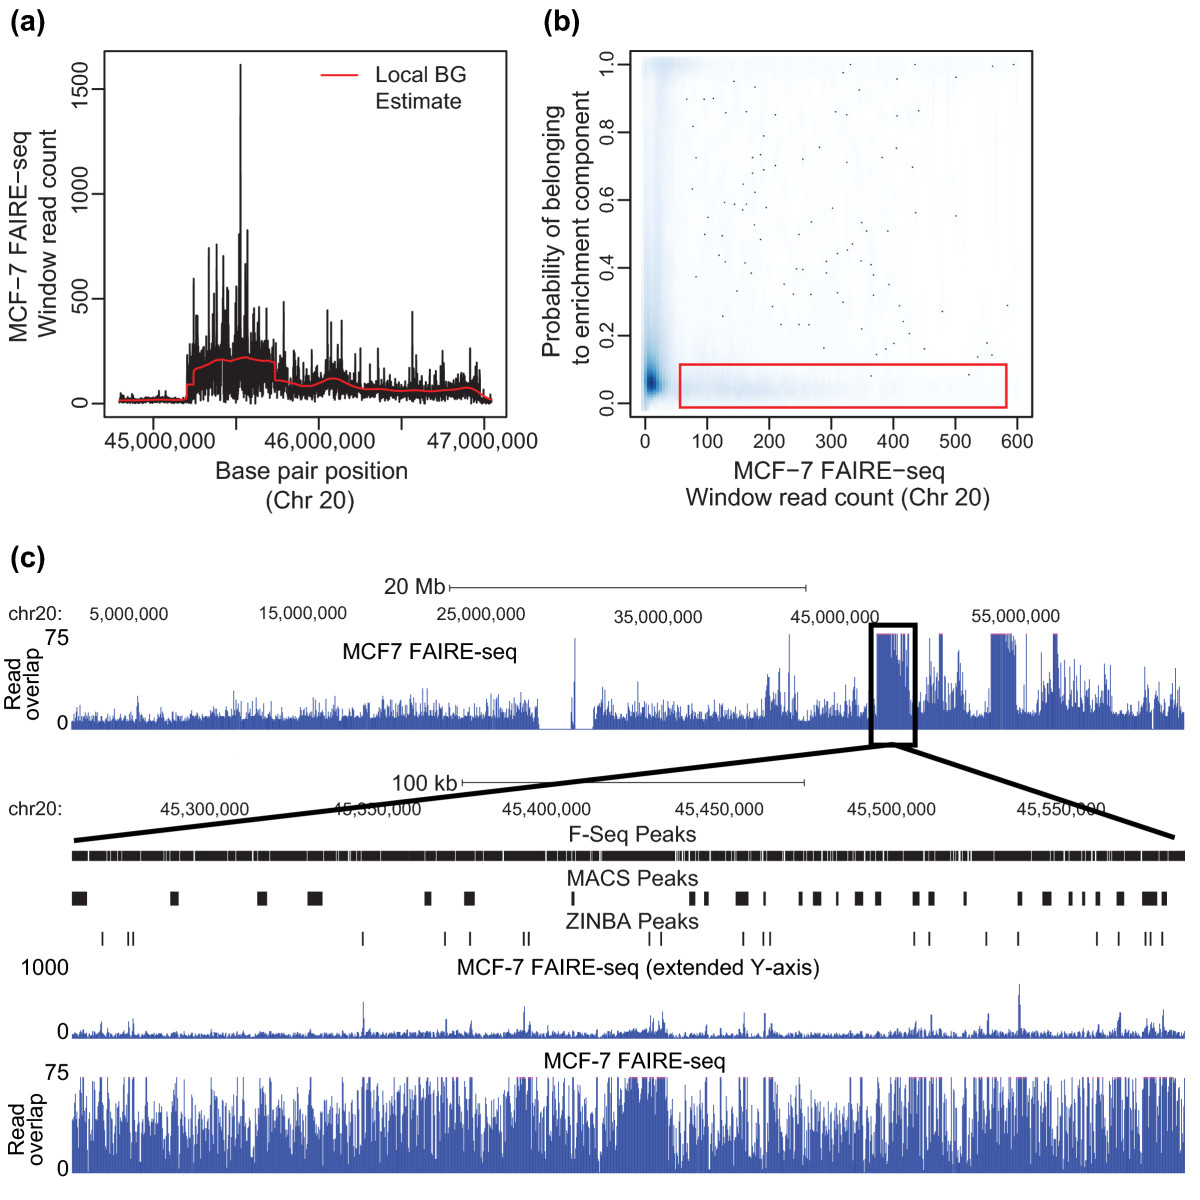
\epsfig{file = ../Figures/RGI12-Fig4.eps, clip=,
	  bbllx=0, bblly=108.2, bburx=260, bbury=139, width=1\textwidth} \\
  \refer{RGI12}

  \bigskip
  \paragraph{Data.}
  $$
  Y_t = \text{number of mapped reads starting at nucleotide $t$}
  $$	
  \ra 'depth of coverage', 'read depth'.
  }

%====================================================================
\frame{\frametitle{CNV detection using microrray}

  $$
    \begin{tabular}{ccc}
%\multicolumn{3}{c}{Zoom on CGH profile} \\
      chrom. 1 & \quad & chrom. 17 \\
      \begin{tabular}{c}
	\epsfig{file = ../Figures/Karyotype-CGH-PH.ps, clip=,
	    bbllx=80, bblly=617, bburx=150, bbury=700, height=.5\textheight}
      \end{tabular}
	& &
      \begin{tabular}{c}
	  \epsfig{file = ../Figures/Karyotype-CGH-PH.ps, clip=,
	    bbllx=270, bblly=617, bburx=300, bbury=700, height=.5\textheight}
	\end{tabular}
      \end{tabular} 
  $$
  \refer{Hup08}
  
  
  \bigskip
  \paragraph{Data.}
  $$
  Y_t = \text{log-fluoresence ratio at probe $t$}
  $$	
}

%====================================================================
\frame{\frametitle{Genome re-arrangement}

  \hspace{-.5cm}
  \begin{tabular}{ccccc}
    \multicolumn{3}{c}{Zoom on CGH profile} & \quad & Karyotype \\
    chrom. 1 & \quad & chrom. 17 \\
    \begin{tabular}{c}
      % \epsfig{file = ../Figures/Karyotype-CGH-PH.ps, clip=,
      % bbllx=80, bblly=617, bburx=150, bbury=763, scale=2}
      \epsfig{file = ../Figures/Karyotype-CGH-PH.ps, clip=,
        bbllx=80, bblly=617, bburx=150, bbury=700, height=.5\textheight}
    \end{tabular}
    & &
    \begin{tabular}{c}
      % \epsfig{file = ../Figures/Karyotype-CGH-PH.ps, clip=,
      % bbllx=270, bblly=617, bburx=300, bbury=763, scale=2}
      \epsfig{file = ../Figures/Karyotype-CGH-PH.ps, clip=,
        bbllx=270, bblly=617, bburx=300, bbury=700, height=.5\textheight}
    \end{tabular}
    & &
    \begin{tabular}{c}
      \epsfig{file = ../Figures/Karyotype-CGH-PH.ps, clip=,
        bbllx=364, bblly=617, bburx=485, bbury=763, height=.5\textheight}
    \end{tabular}
  \end{tabular}

%   \bigskip
%   Pair-end allows to capture re-arrangement, whereas $Y_t$ alone does not.
}

%====================================================================
\frame{\frametitle{Gene discovery with RNA-seq}

    \begin{tabular}{cc}
      \hspace{-.5cm}	
      \begin{tabular}{p{.4\textwidth}}
	\paragraph{Data.} \\
      $Y_t =$ number of mapped reads starting at nucleotide $t$
	~\\
      \end{tabular}
      &
      \hspace{-.5cm}	
      \begin{tabular}{p{.5\textwidth}}
	RNA-seq counts \\
	~\\
	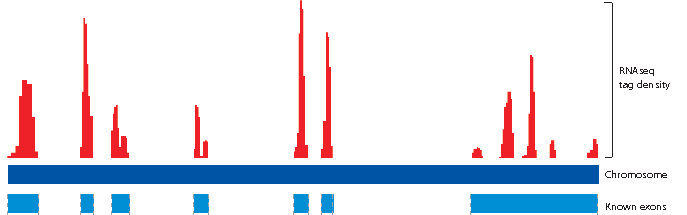
\epsfig{file=../Figures/gb-2008-9-9-234-1.eps,
	  width=.5\textwidth, height=.3\textheight, bbllx=0,
	  bblly=275, bburx=300, bbury=425, clip=} \\
	~\\
	Known exons \\
	~\\
	source: \Refer{genomebiology.com}
      \end{tabular}
    \end{tabular}
}

%====================================================================
\subsection*{(Statistical) questions}
%====================================================================
\frame{\frametitle{Segmentation: the basic problem}
  
  %\vspace{-0.5cm}
  \begin{tabular}{cc}
    \begin{tabular}{p{.5\textwidth}}
      \onslide+<1->{
        \paragraph{Data at hand:} for a given individual
        \begin{itemize}
        \item a sequence of \emphase{known positions} along the
          \emphase{reference genome}, labeled as
          \[
          t = 1, 2, \dots, n
          \]
        \item a signal measured \emphase{at each position}
          \[
          Y_t = \text{signal at position $t$}
          \]
        \end{itemize}
        }
    \end{tabular}
    &
    \begin{tabular}{p{.5\textwidth}}
      \hspace{-1cm}
      \begin{overprint}
        \onslide<2-3>
        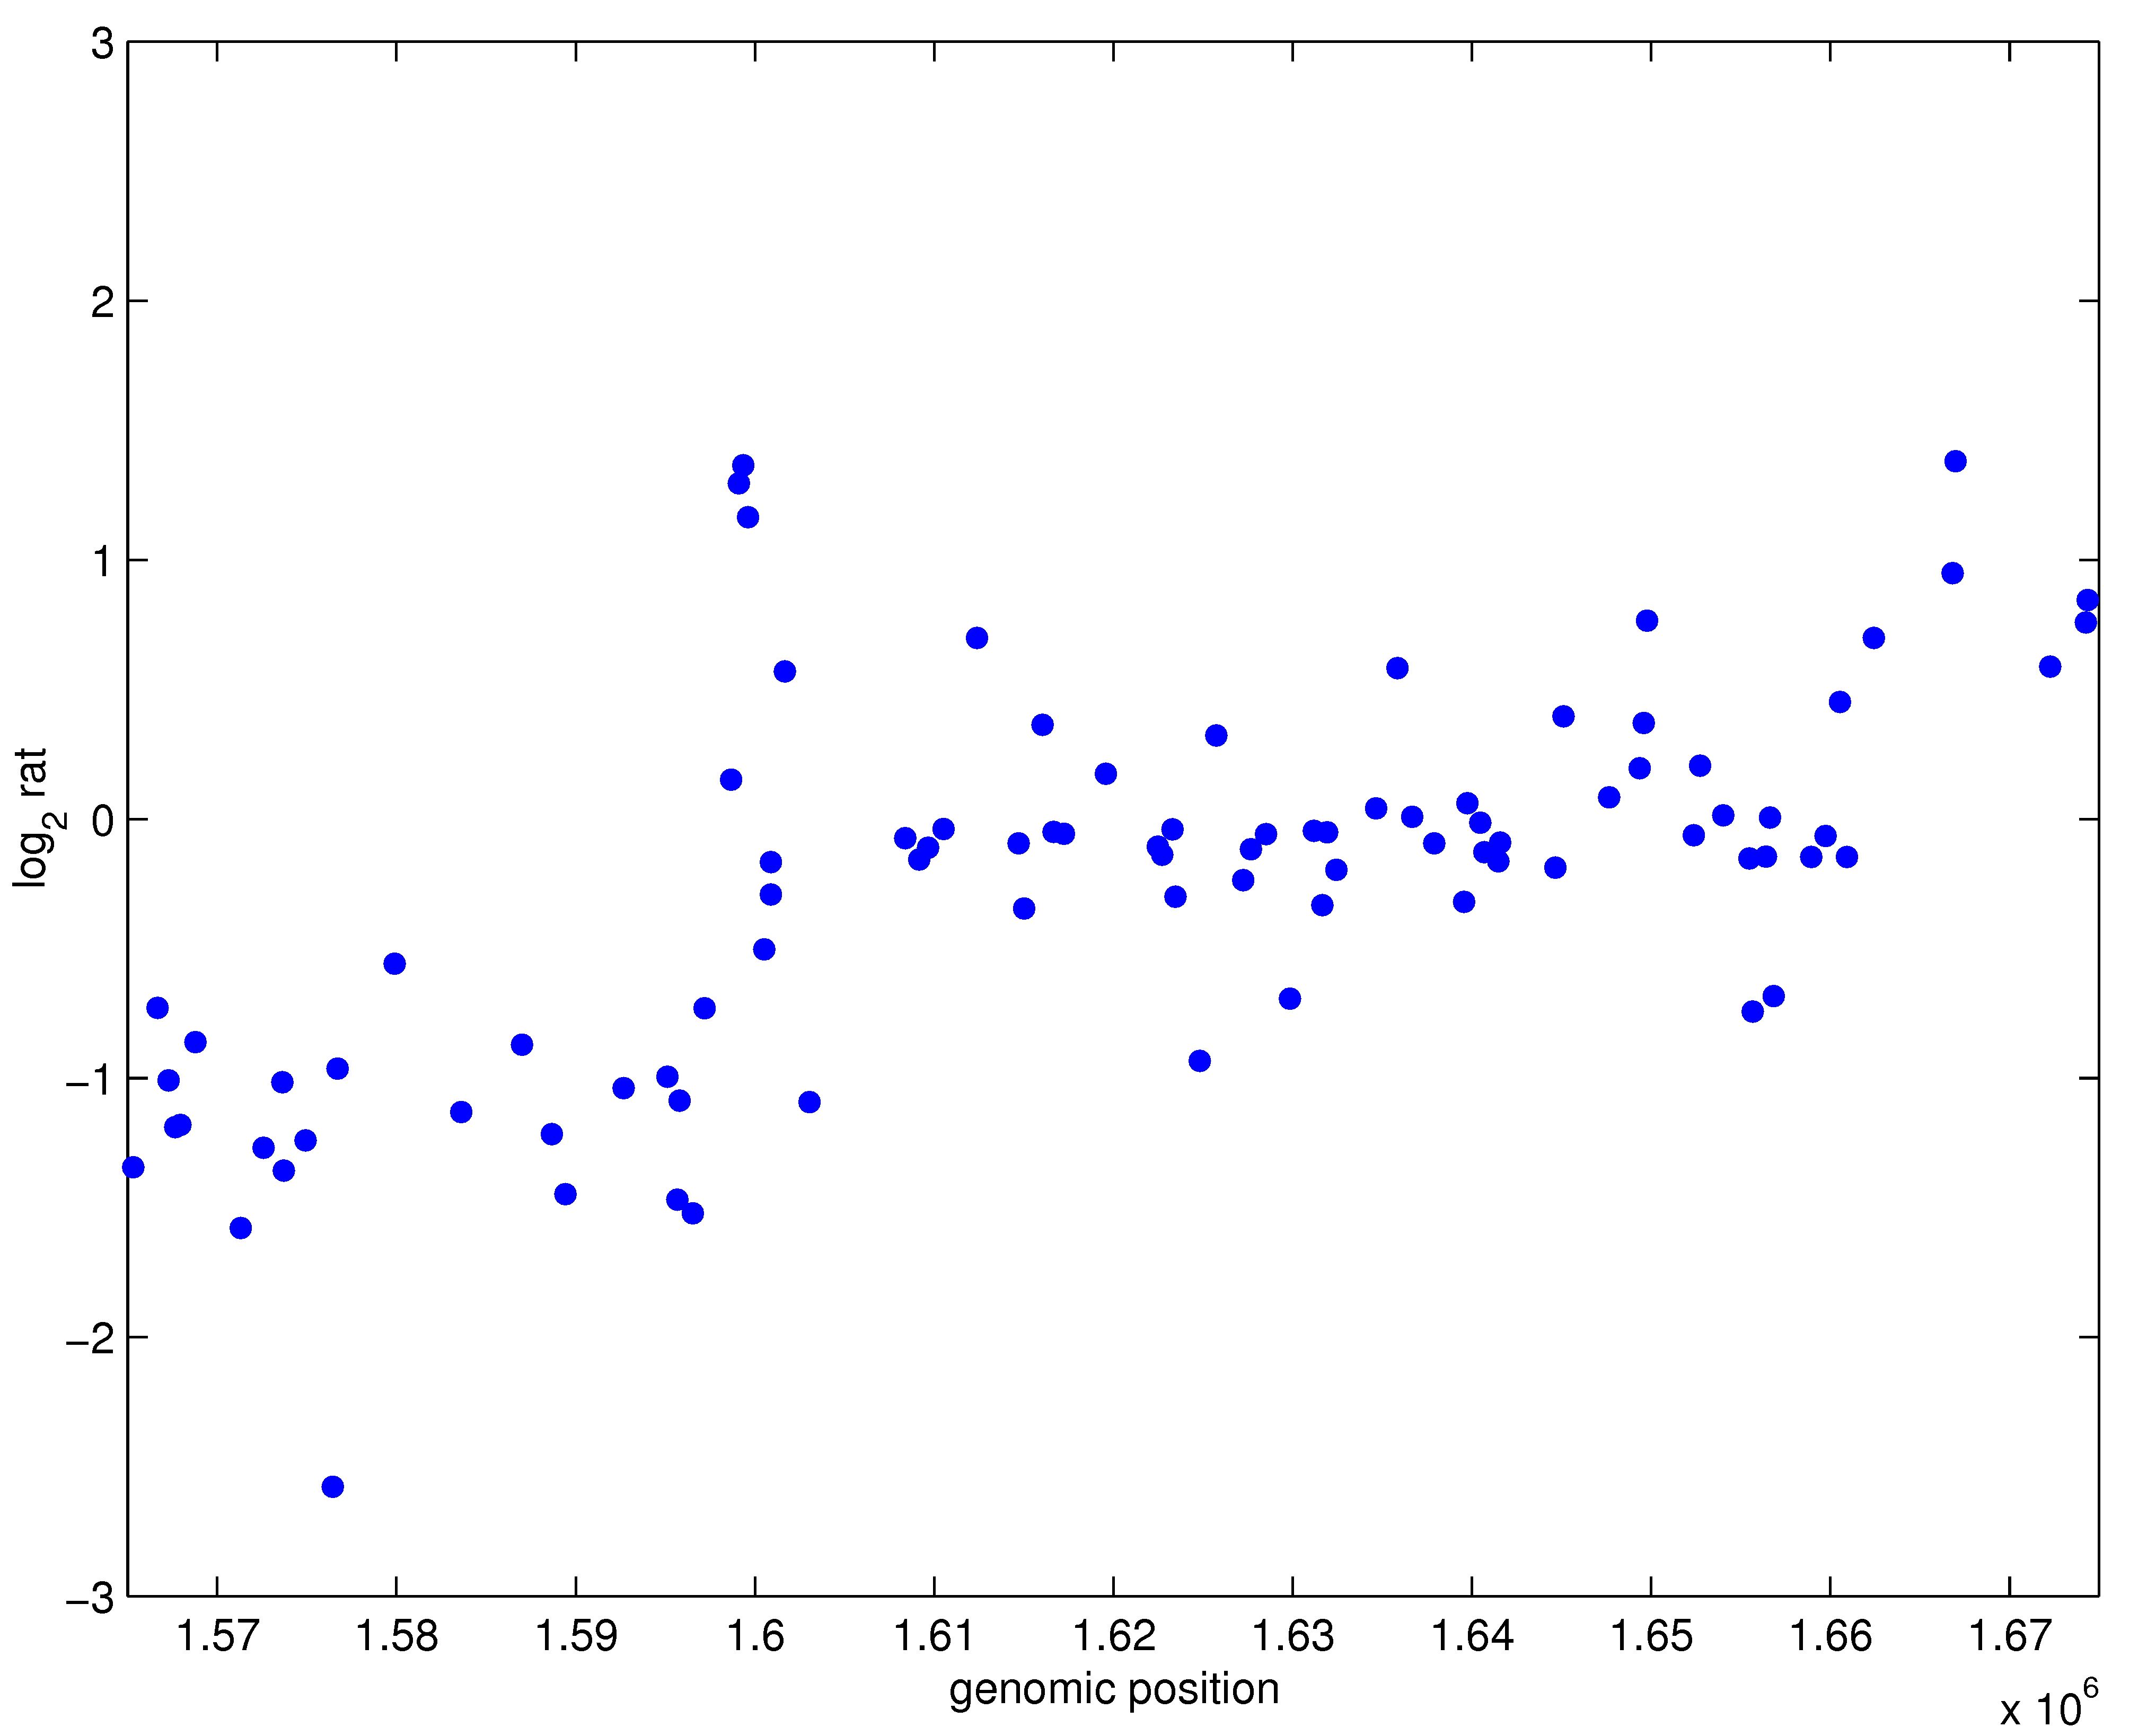
\epsfig{file = ../Figures/raw_profile_example.eps, clip=,
          width=.45\textwidth, height=.5\textheight}  
        \onslide<4>
        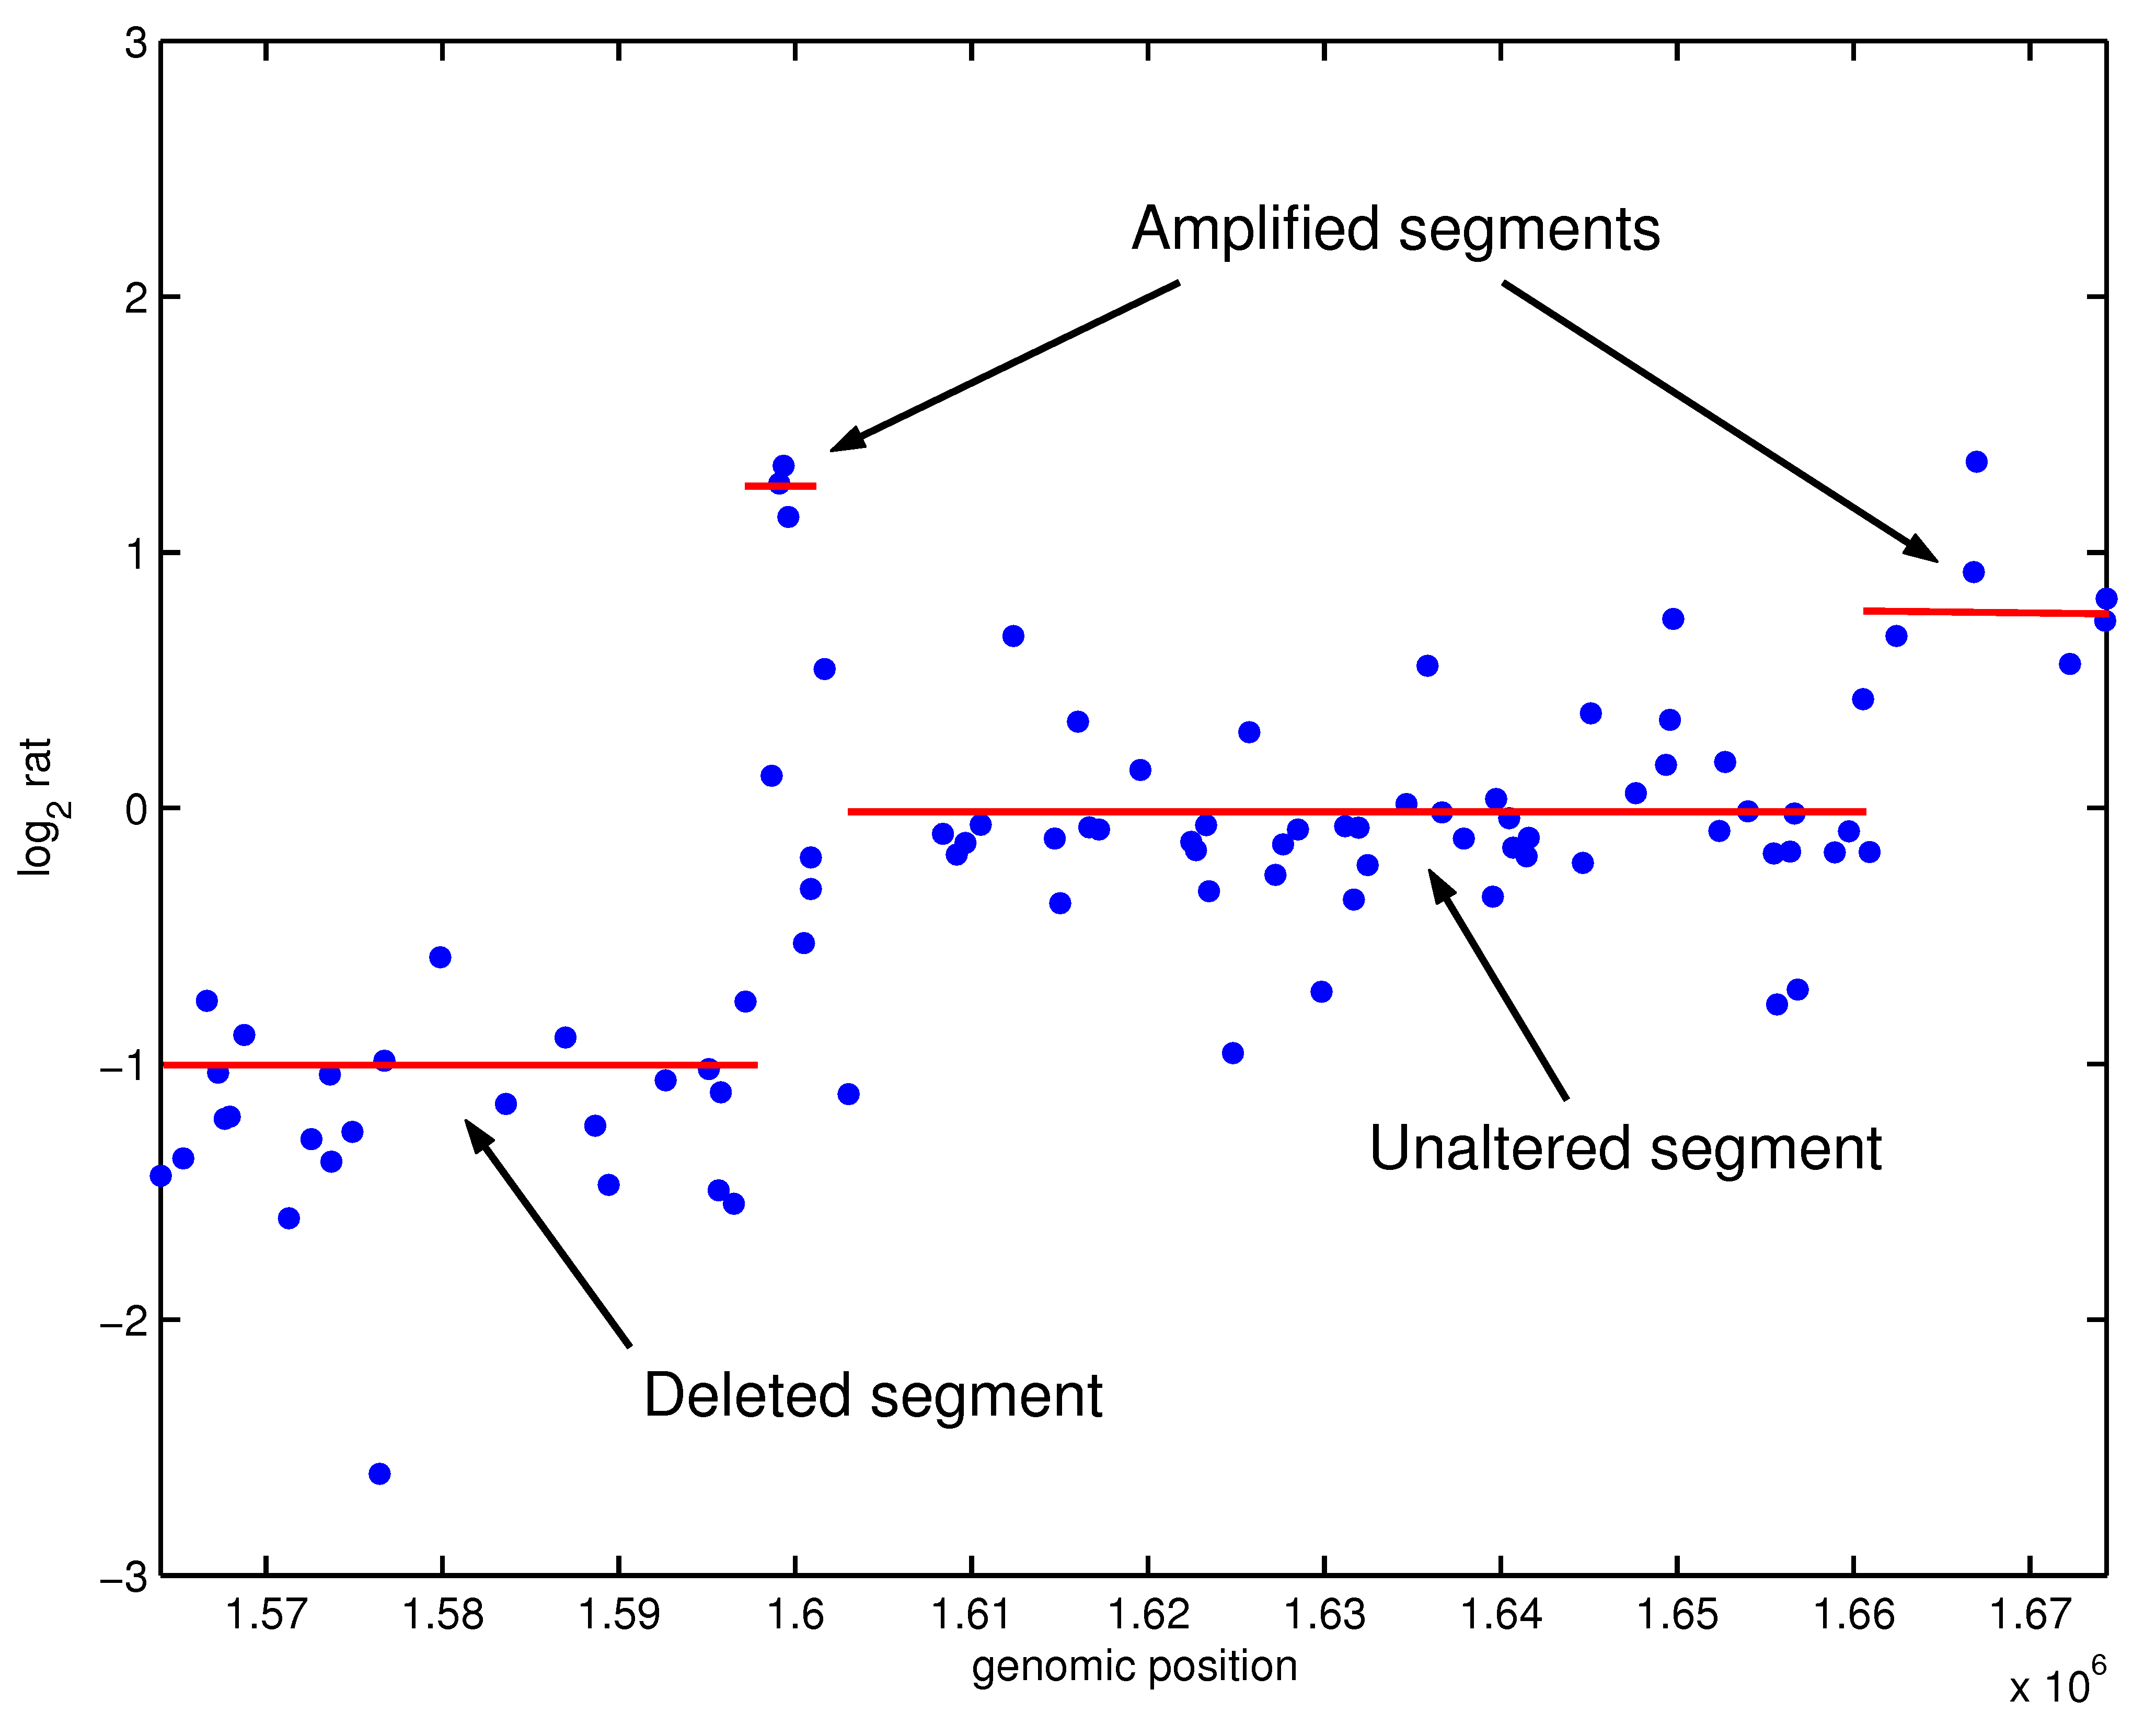
\epsfig{file = ../Figures/profile_example.eps, clip=,
          %bbllx=60, bblly=196, bburx=543, bbury=586}
          width=.45\textwidth, height=.5\textheight}  
      \end{overprint}
    \end{tabular}
  \end{tabular} \\
  \onslide+<3->{
    \begin{eqnarray*}
      Y_t & \propto & f(\text{\emphase{relative copy number} at position }t) \\
      & = & \text{DNAseq count, log-fluorescence, etc.}
    \end{eqnarray*}
    }
  }

%====================================================================
\frame{\frametitle{Example: Breast cancer CGHarray}

  \vspace{-.5cm}
  \[
  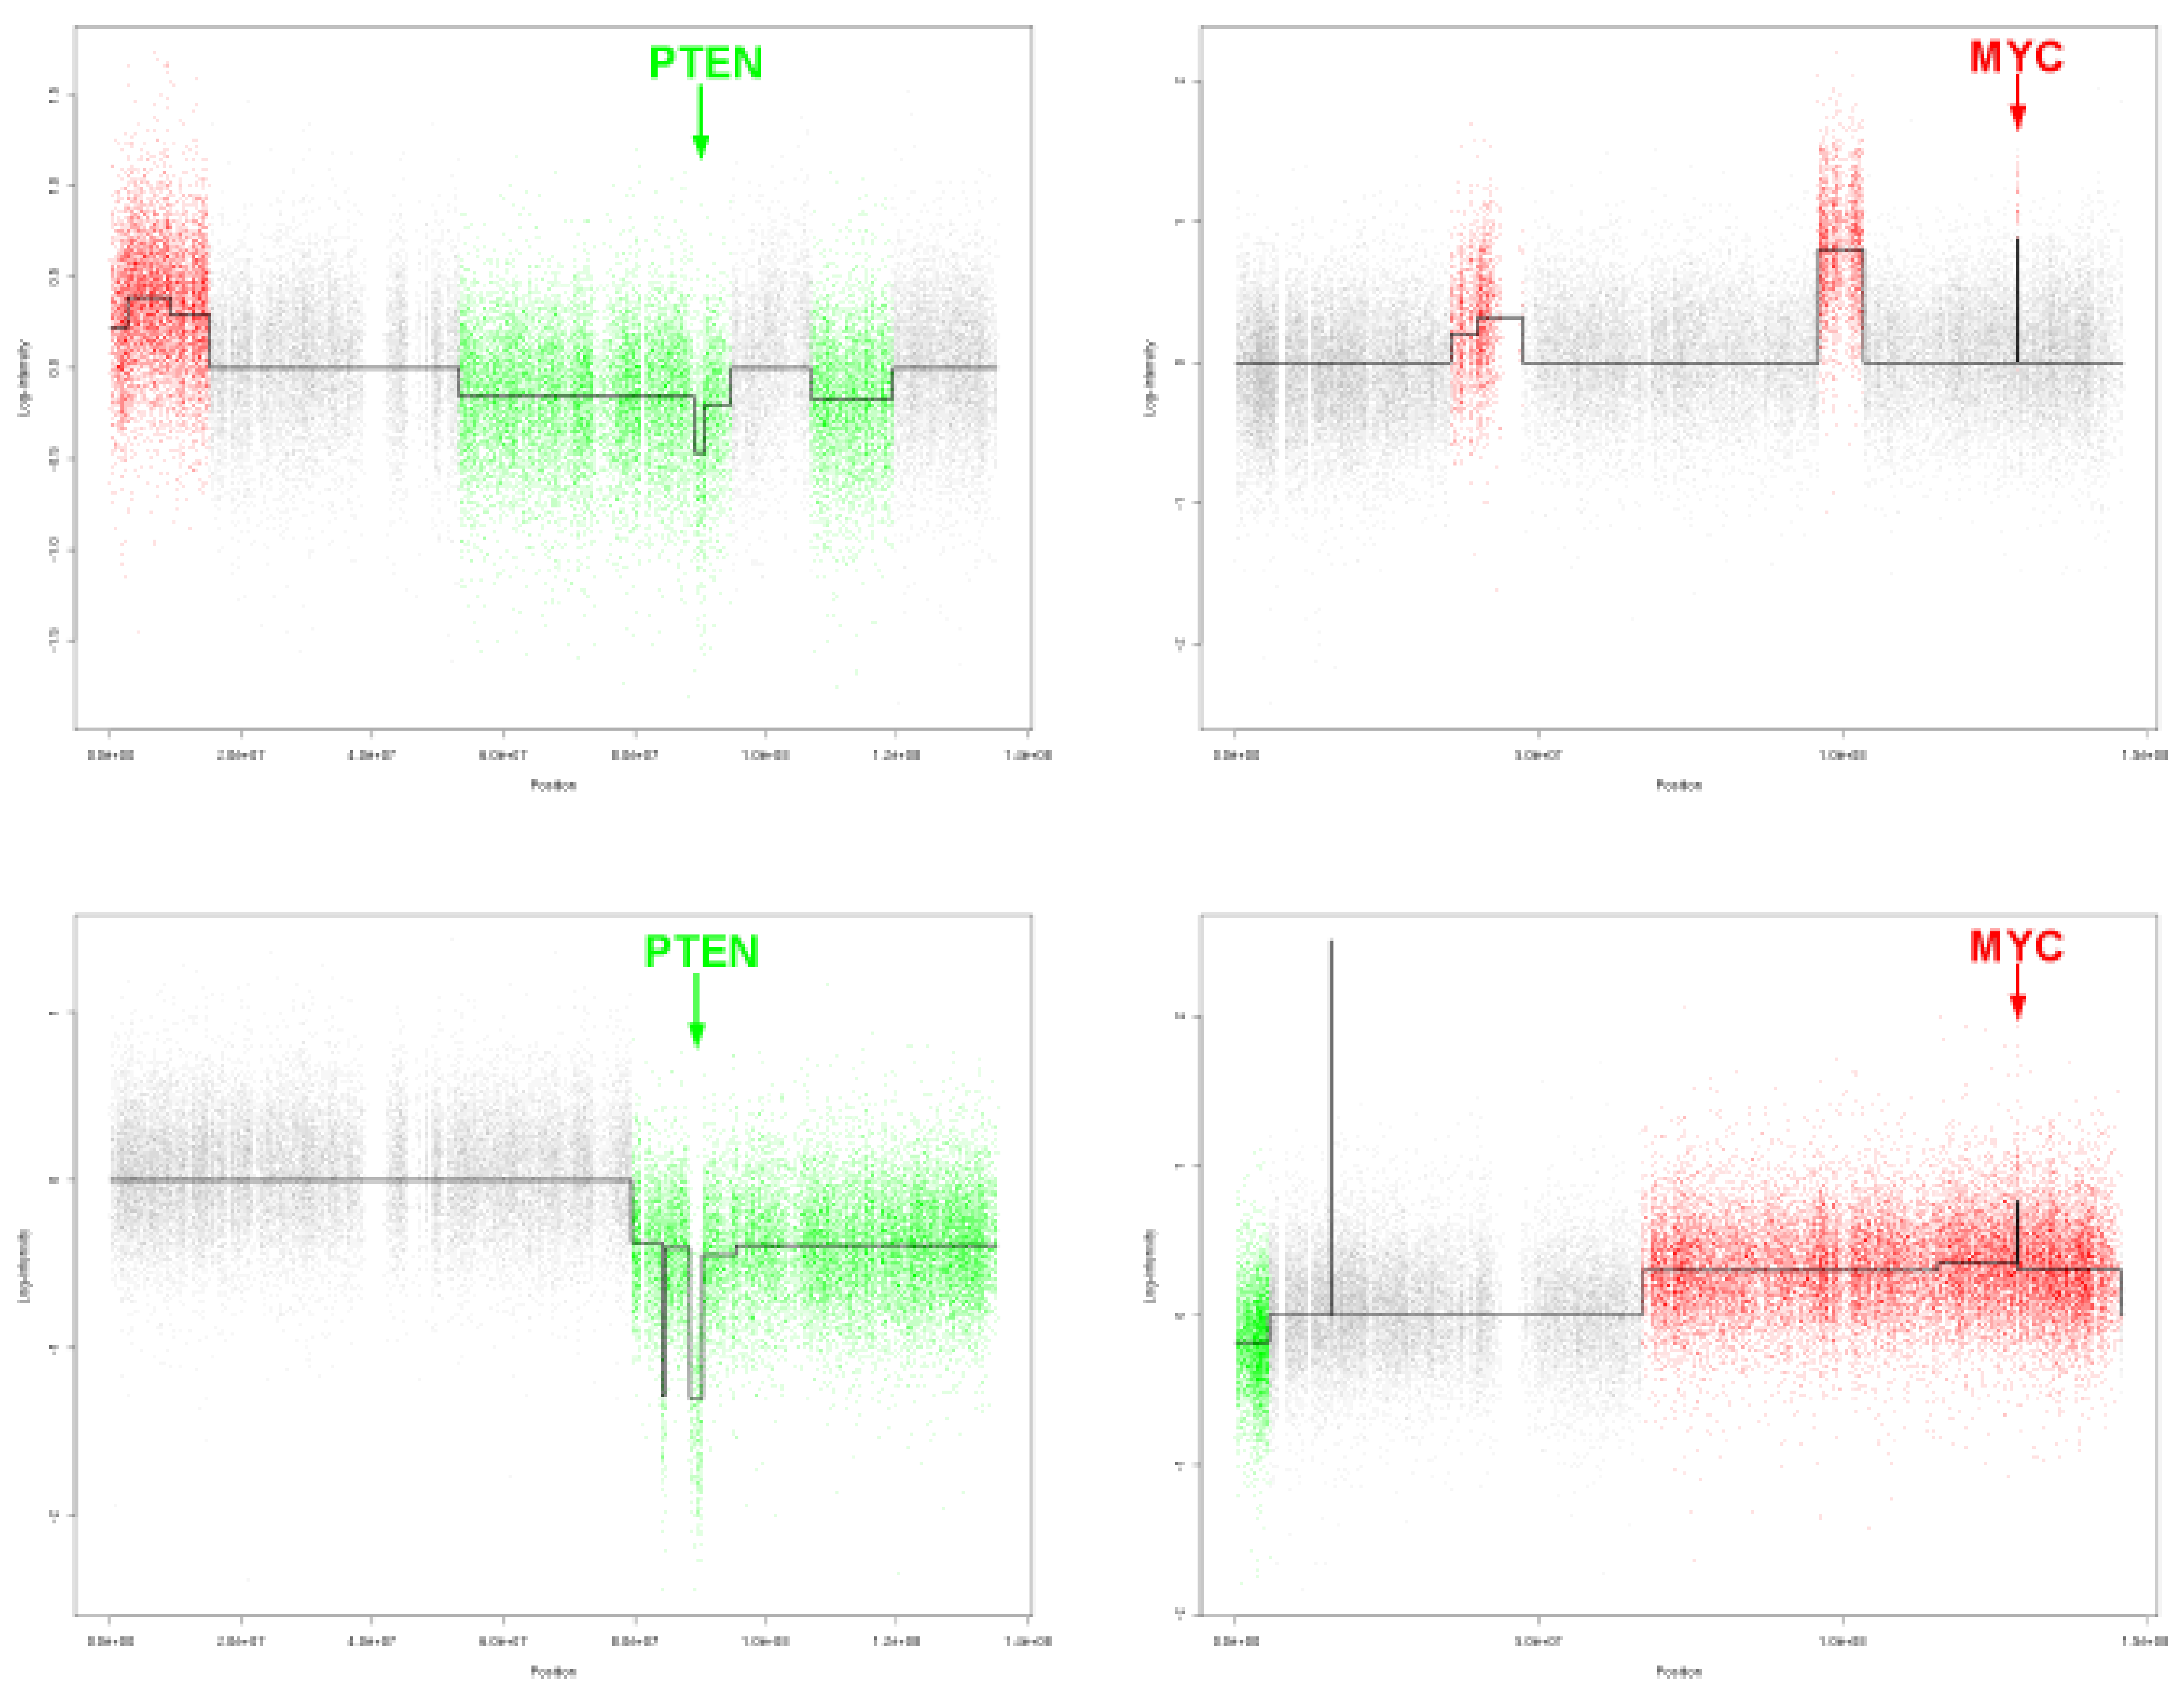
\epsfig{file = ../Figures/Rig10-Fig6-5.ps, height=.8\textheight,
    width=.8\textwidth} 
  \] 
  Chrom. 10 and 8 of two breast carcinomas (TNBC). \refer{Rig11} 
}\label{Page:BreastCancer}

%====================================================================
\frame{\frametitle{(Statistical) questions}
  
  \paragraph{Biological questions:}  
  \begin{itemize}
  \item How many change points?
  \item Where are the change points? (How precise is the location?)
  \item Do the change points have the same location in samples $A$
    and $B$?
  \item ...
  \end{itemize}
  
  \bigskip\pause
  \paragraph{Statistical issues:}  
  \begin{itemize}
  \item Statistical modeling
  \item Computational efficiency
  \item Model selection
  \end{itemize}
}

%====================================================================
\frame{\frametitle{Data specificities}

  \paragraph{Dimension.}
  \begin{itemize}
   \item Whole chromosome CNV detection using DNAseq \ra $n = 10^8$
   \item Whole chromosome CNV detection using SNParray \ra $n = 10^6$
   \item 'Small' gene reannotation  using RNAseq \ra $n = 10^4$
  \end{itemize}
  \ra Different computational burdens.

  \bigskip \pause
  \paragraph{Stucture.}
  \begin{itemize}
   \item One measurement per position (probe or nucleotide)
   \item Pairs of positions (pair-end) \ra \emphase{out of my scope}\footnote{Are statisticians slower than computer scientists?}
  \end{itemize}
  
  \bigskip \pause
  \paragraph{Nature.}
  \begin{itemize}
   \item Microarray \ra fluorescence \ra continuous data ($\in \Rbb$)
   \item NGS \ra read counts \ra discrete data ($\in \Nbb$)
  \end{itemize}

}

%====================================================================
%====================================================================
\section{Segmentation methods}
\frame{\frametitle{Segmentation methods}}
%====================================================================

%====================================================================
\subsection*{Statistical model}
%====================================================================
\frame{\frametitle{A model, what for?}
  
  \begin{itemize}
  \item To \emphase{translate biological questions into mathematical
      equations} and quantities;
  \item To make \emphase{all hypotheses explicit};
  \item To set the inference of interesting parameters in a
    \emphase{global framework}, possibly accounting for other effects
    (covariates);
  \item To \emphase{motivate all calculations} and data processing to
    come.
  \end{itemize}
  
  \bigskip\pause
  \centerline{\emphase{The model is the place where biologist's and
      mathematician's minds meet.}}
  
  \bigskip\bigskip\pause
  \paragraph{Model-based approach.}
  \begin{itemize}
  \item Define a model that describes the biological process as well
    as possible;
  \item Make sure that it can be handled in terms of mathematics /
    statistics;
  \item Derive an (efficient and statistically valid) inference
    procedure.
  \end{itemize}
}

%====================================================================
\frame{\frametitle{Segmentation model}

  \begin{tabular}{cc}
    \hspace{-.5cm}
    \begin{tabular}{p{.5\textwidth}}
      \onslide+<2->{\paragraph{Statistical model.} 
        \begin{itemize}
        \item $\text{Signal} = f(\text{Position})$; \\}
        \onslide+<3->{
        \item Breakpoint positions: \\
          $\tau_1, \tau_2, ..., \tau_{K-1};$ \\}
        \onslide+<4->{
        \item 'Mean' signal (e.g. copy number) within each interval: \\
          $\mu_1, \mu_2, ..., \mu_K$; \\}
        \onslide+<5->{
        \item Observed signal at time $t$: \\
          independent variables with given parameter (mean, dispersion, ...).
        \end{itemize}}
    \end{tabular}
    & 
    \hspace{-1cm}
    \begin{tabular}{c}
      \onslide+<2->{
        \hspace{-6cm}
        \onslide+<3->{if $t \in \textcolor{blue}{r_k}$,} \quad $Y_t$
        \onslide+<5->{$\sim
          \Fcal($}\onslide+<4->{$\textcolor{red}{\mu_k}$}\onslide+<5->{$)$}
        \\}
      \begin{overprint}
        \onslide<2>
%        $\qquad \qquad \;\;\, Y_t =$ \\
        \epsfig{file=../Figures/FigSeg-Budapest-1.eps, clip=,
          angle=270, width=.5\textwidth} 
        \onslide<3>
%        if $t \in \textcolor{blue}{r_k}, \quad Y_t$ \\
        \epsfig{file=../Figures/FigSeg-Budapest-2.eps, clip=,
          angle=270, width=.5\textwidth} 
        \onslide<4>
%        if $t \in \textcolor{blue}{r_k}, \quad Y_t \textcolor{red}{\mu_k}$ \\
        \epsfig{file=../Figures/FigSeg-Budapest-3.eps, clip=,
          angle=270, width=.5\textwidth} 
        \onslide<5->
%        if $t \in \textcolor{blue}{r_k}, \quad Y_t \sim
%        \Fcal(\textcolor{red}{\mu_k})$ \\ 
        \epsfig{file=../Figures/FigSeg-Budapest-4.eps, clip=,
          angle=270, width=.5\textwidth} 
      \end{overprint}
    \end{tabular}
  \end{tabular}

%   \onslide+<6->{
%     \paragraph{Possible choices for the distribution $\Fcal$:} 
%     \begin{itemize}
%     \item CGHarray: continuous signal (fluorescence) \ra Gaussian distribution;
%     \item NGS: discrete signal (counts) \ra Poisson or negative
%       binomial distribution.
%     \end{itemize}
%   }
}

%====================================================================
\frame{\frametitle{Dealing with (some) data specificities} 
  
  \paragraph{Distribution.} The distribution $\Fcal$ of the data is chosen according to the technology:
    $$
    \begin{array}{c}
      \text{if position $t$} \\
      \text{is in segments $r_k$:}
    \end{array}
    \quad 
    \left\{ 
      \begin{array}{rcll}
        Y_t & \sim & \Ncal(\mu_k,\sigma^2)  & \text{aCGH (same
          variance)} \\
        \\
%         Y_t & \sim & \Ncal(\mu_k,\sigma_k^2)  & \text{aCGH (heter.
%           variance)} \\  
%         \\
        Y_t & \sim & \Pcal(\mu_k)  &  \text{NGS} \\
        \\
        Y_t & \sim & \Ncal\Bcal(\mu_k, \phi)  &  \text{NGS (over-dispersed)}
      \end{array}
    \right.
    $$

    \bigskip \pause
    \paragraph{Normalization?}
    {Explicit modeling allows to account for additional information}, e.g. $x_t =$ GC content at position $t$:
    $$
    Y_t \sim \Ncal(\mu_k + \lambda x_t, \sigma^2)
    $$	
    (see CGHseg package later on).
  }

%====================================================================
\frame{\frametitle{Data transformation}

  \begin{itemize}
  \item The reference distributions for NGS data are Poisson and negative binomial for which many methods are being developped. \\~
  \item \pause Many methods exist for continuous data (Gaussian, as usual, easier to handle). \\~
  \item \pause Data transformation could be used to apply them to NGS data, e.g.:
  $$
  \widetilde{Y}_t = \log(1 +  Y_t), 
  \qquad
  \widetilde{Y}_t = \sqrt{Y_t}, 
  $$
  \item \pause Reminder: the variance stabilizing transformation for the negative binomial is 
  $$
  \widetilde{Y}_t = \arg\sinh \sqrt{\frac{Y_t}{\phi}}
  $$	
  \end{itemize}
}

%====================================================================
\subsection*{Parameter inference}
%====================================================================
\frame{\frametitle{Parameter inference}

  \paragraph{Two different types of parameters of the models:}
  \begin{itemize}
  \item Segmentation (change point locations): $T = (\tau_1, \dots,
    \tau_{K-1})$ \\
    \ra discrete parameter;
  \item Distribution parameters (within segment means): $\mubf =
    (\mu_1, \dots, \mu_K)$ \\
    \ra continuous parameter.
  \end{itemize}

  \bigskip\bigskip\pause
  \paragraph{Fitting model to data:} The estimates of $T$ and $\mu$ are expected to provide a good fit to the data.
  \begin{enumerate}
   \item Define a criterion to measure this fit
   \item Find the 'optimal' values $\widehat{T}$ and $\widehat{\mubf}$ providing the best fit.
  \end{enumerate}

}

%====================================================================
\frame{\frametitle{Maximum likelihood}

  \paragraph{Most common strategy: Maximum likelihood}
  To get estimate of the parameters of this model ($T, \mubf$)
  we choose to maximize the likelihood of the observed data:
  \begin{eqnarray*}
  p(\Ybf; T, \mubf) & = & \textcolor{red}{\prod_k} \textcolor{blue}{\prod_{t \in r_k}} p(Y_t; \mu_k) \\
  \Rightarrow \qquad \log p(\Ybf; T, \mubf) & = & \textcolor{red}{\sum_k}
  \textcolor{blue}{\sum_{t \in r_k}} \log p(Y_t ;\mu_k).
  \end{eqnarray*}

  \bigskip\pause
  \paragraph{Array CGH.} Gaussian with same variance $\Ncal(\mu_k, \sigma^2)$:
  $$
  \log P(\Ybf; T, \mubf) = \text{cst} - \text{cst} \sum_k \sum_{t \in r_k} (Y_t - \mu_k)^2
  $$
  
  \bigskip\pause  
  \paragraph{NGS.} Poisson $\Pcal(\mu_k)$:
  $$
  \log P(\Ybf; T, \mubf) = \text{cst} - \sum_k \sum_{t \in r_k}
  (\mu_k - Y_t \log \mu_k)
  $$

  }
  
%====================================================================
\frame{\frametitle{Parameter inference} 

  \paragraph{When the breakpoints are known,} estimating the
  parameters is (generally) an easy task, e.g. for the mean
  $$
  \widehat{\mu}_k = \frac1{n_k} \sum_{t \in r_k} Y_t
  $$

  \pause\bigskip
  \paragraph{Finding the breakpoints:} We now have to find the change-points $T = (\tau_1, \dots, \tau_{K-1})$ that maximize the log-likelihood
  $$
  \log p(\Ybf; T) = \sum_k  \sum_{t \in r_k} \log p(Y_t ;\widehat{\mu}_k).
  $$
  \pause\bigskip
  \paragraph{Problem.} There are $ \binom{n-1}{K-1} $ possible choices
  for the positions of the breakpoints $\tau_1, \tau_2, \dots,
  \tau_{K-1}$.
  $$
  \text{For } n=1\,000, \qquad K = 20 \quad \longrightarrow \quad
  \binom{n-1}{K-1} \simeq 10^{40}
  $$
  \ra Impossible to explore for large $n$ and $K$

}\label{Page:ParamInfer}

%====================================================================
\subsection*{Dynamic programming}
%====================================================================
%====================================================================
\frame{\frametitle{Shortest path problem}

  \paragraph{Cost of segment.} Define the cost of segment $r= [i, j]$ as
  $$
  C(i, j) = C(r) = \sum_{t \in r} - \log p(Y_t; \widehat{\mu}_r),    
  $$
  finding the maximum likelihood segments
%   the maximization of
%   $$
%   \log p(\Ybf; T) = \sum_k  \sum_{t \in r_k} \log p(Y_t; \widehat{\mu}_k).
%   $$
  can be restated as a \paragraph{shortest path problem}, that is to find the path
  \begin{itemize}
  \item going from 1 to $n$,
  \item in $K$ steps,
  \item for the best possible cost.
  \end{itemize}

  \pause \bigskip
  \paragraph{Exact solution.} This shortest path problem can be solve \emphase{exactly}
  thanks to a dynamic programming algorithm with complexity
  \begin{itemize}
  \item $O(K n^2)$ for computational time and
  \item $O(Kn)$ for memory space.
  \end{itemize}
 }

%====================================================================
\frame{\frametitle{Fastening the DP algorithm}

  \paragraph{Quadratic complexity} $O(Kn^2)$ is not acceptable for very
  large signals ($n = 10^8$).

  \pause\bigskip
  \begin{tabular}{cc}
    \hspace{-.5cm}
    \begin{tabular}{p{.5\textwidth}}
      The computational time can be reduced to almost linear ($O(K n \log n)$). \\
      ~\\
      \emphase{Pruned DPA:} (\refer{Rig10}) relies on an algebraic trick\footnote{Not to compute parameter estimates (see slide \ref{Page:ParamInfer}) before to perform segmentation \ra only applicable for 'nice' contrasts}. \\
      ~\\
      \emphase{PELT:} (\refer{KFE11}) takes advantage of the penalty to simplify the contrast.
      ~\\
    \end{tabular}
    &
    \hspace{-.5cm}
    \begin{tabular}{p{.5\textwidth}}
    \epsfig{file = ../Figures/Rig10-Fig.ps, clip=, bbllx=290,
      bblly=20, bburx=560, bbury=270, width=.4\textwidth}     
    \end{tabular}
  \end{tabular}
}

%====================================================================
\subsection*{Model selection}
%====================================================================
%====================================================================
\frame{\frametitle{How many change-points?}

  \vspace{-.5cm}
  \begin{tabular}{cc}
    \hspace{-.5cm}
    \begin{tabular}{p{.45\textwidth}}
	  \paragraph{How many segments?}
	  \begin{itemize}
	    \item The number of segments $K$ is not known a priori.
	    \item The fit of the segmentation improves as $K$ 	
		    increases.
	  \end{itemize}
  
	  \bigskip 
	  \paragraph{Penalized likelihood $=$} most common strategy:
	  \[
	  \onslide+<4->{\textcolor{blue}{\widehat{K}} = \arg\min_K}
	  ~\onslide+<2->{- \log p(\Ybf; K)}
	  ~\onslide+<3->{\textcolor{red}{+ \text{pen}(K)}}
	  \]
    \end{tabular}
	&
    \begin{tabular}{p{.5\textwidth}}
	    \begin{overprint}
    	\onslide<2>
	      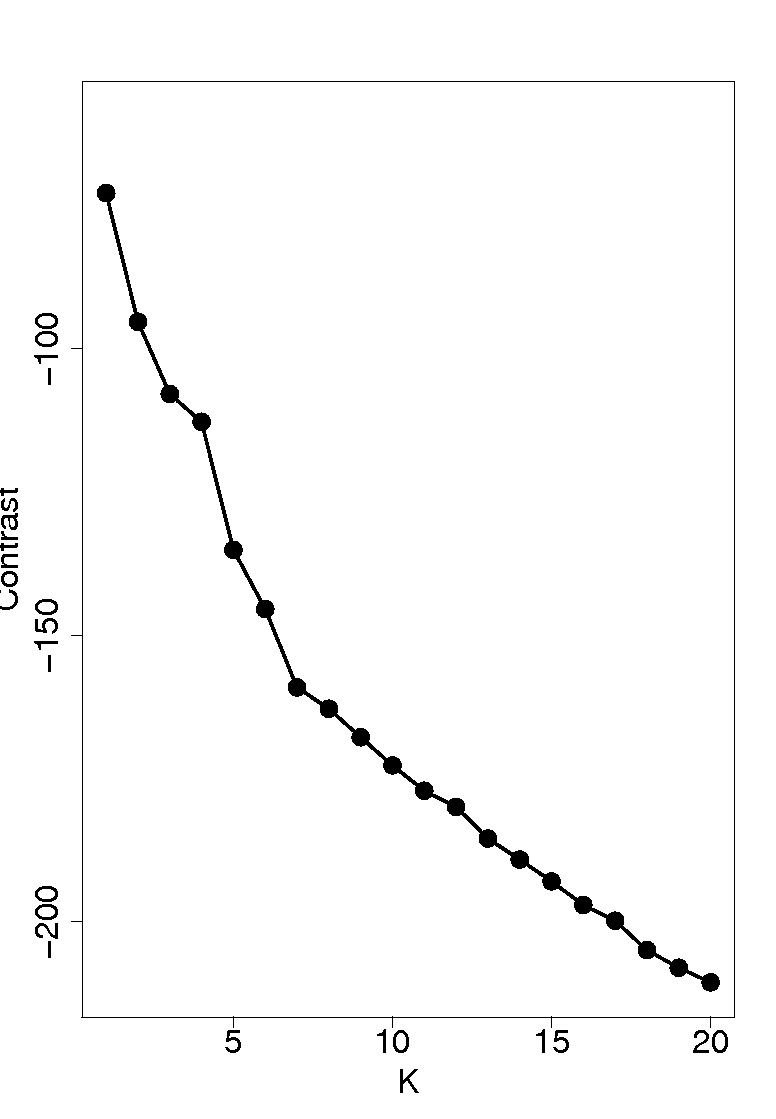
\epsfig{file = ../Figures/Bt474-J.ps, clip=, width=.5\textwidth,
	       height=.7\textheight} 
    	\onslide<3>
	      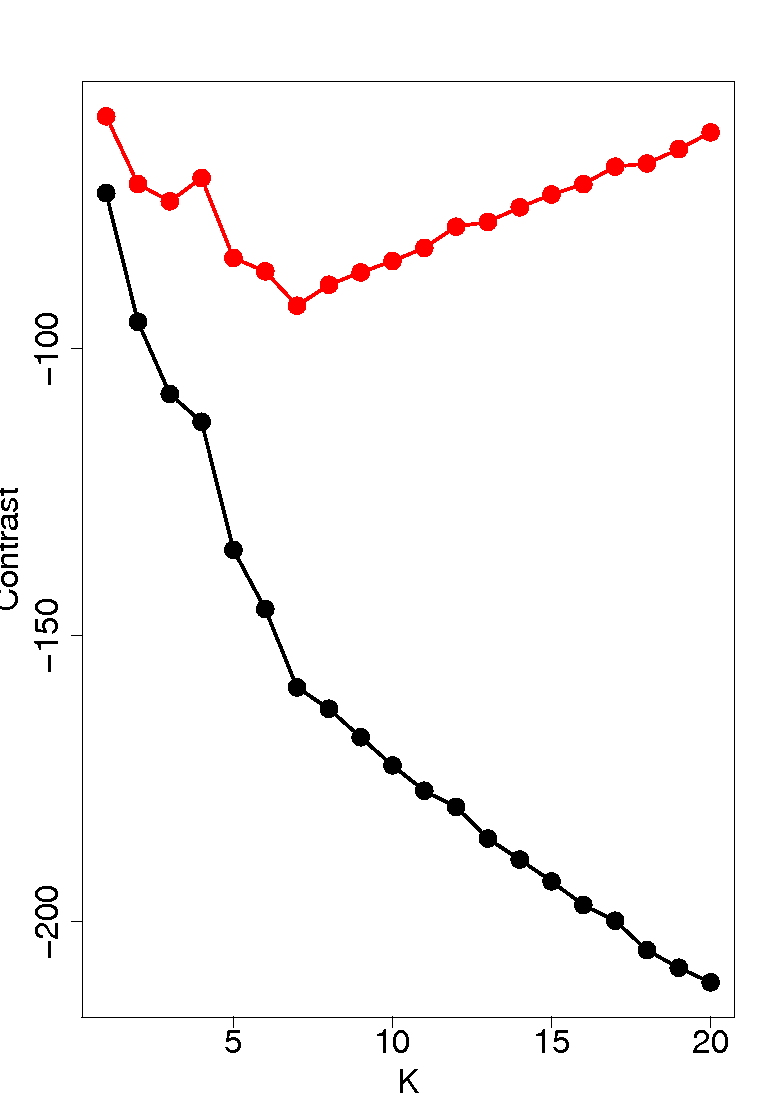
\epsfig{file = ../Figures/Bt474-JP.ps, clip=, width=.5\textwidth,
	       height=.7\textheight} 
    	\onslide<4->
	      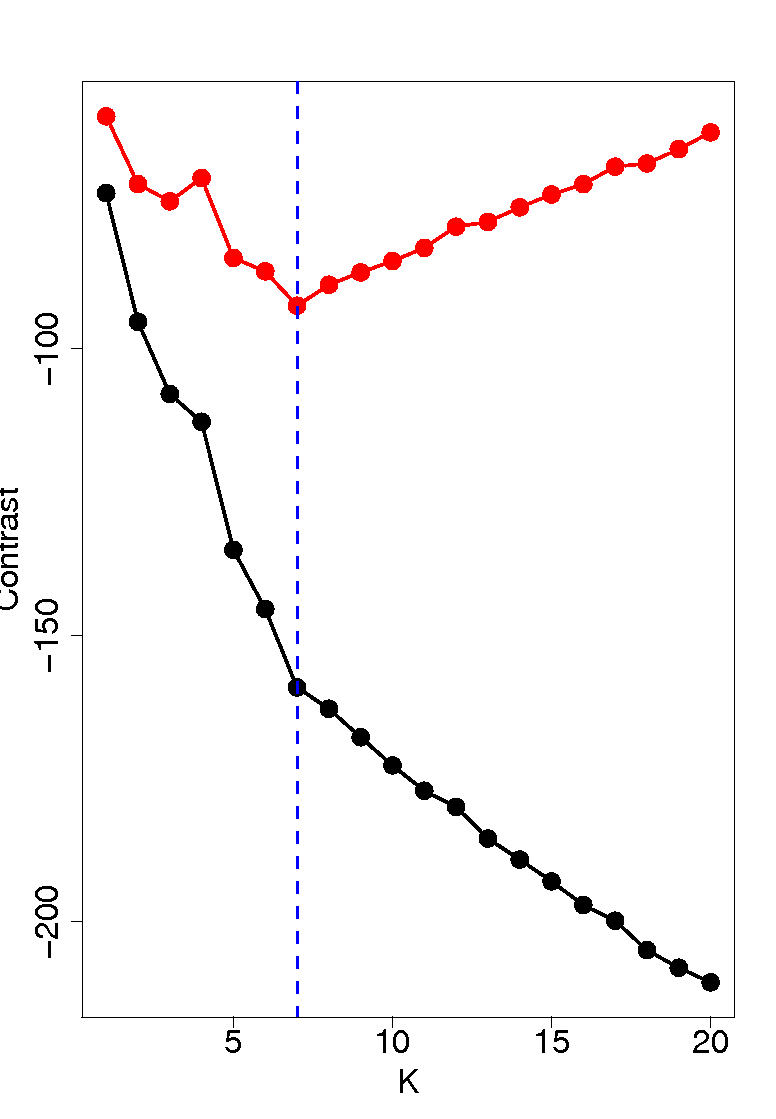
\epsfig{file = ../Figures/Bt474-JPM.ps, clip=, width=.5\textwidth,
	       height=.7\textheight} 
	    \end{overprint}
    \end{tabular} 
  \end{tabular} 

  \onslide+<5>{ 
    \vspace{-.5cm} An abundant literature has been developed
    (\refer{Leb05}, \refer{Lav05}, \refer{ZhS07}, ...) to insure that
    $\Pr\{\widehat{K} = K\} \rightarrow 1$ when $n \rightarrow \infty$
    or to approximate $p(K | \Ybf)$.  }
  
}

%====================================================================
\frame{\frametitle{Penalization}

  Penalty 'calibration' requires theoretical developments, each dedicated to a specific model

  \begin{itemize}
    \item Gaussian homoscedastic (\refer{Leb05}) :  
    $$
    pen(K) = \frac{K}{n} \left(\log\dfrac{n}{K} +2.5\right) 
    $$ 
    \item Negative Binomial (\refer{ClL12}): 
    $$
    pen(K) = \frac{K}n \left(1+4\sqrt{1.1+\log\frac{n}{K}}\right)^2 
    $$
  \end{itemize}
}

%====================================================================
\subsection*{In practice}

%====================================================================
\frame{\frametitle{Comparative study (for CGH)}

  Based on \emphase{manually annotated CGH profiles}, ROC curves can be drawn to compare the performances of a series methods, in terms of change-point detection (\refer{Hoc12}). \\
  \pause
  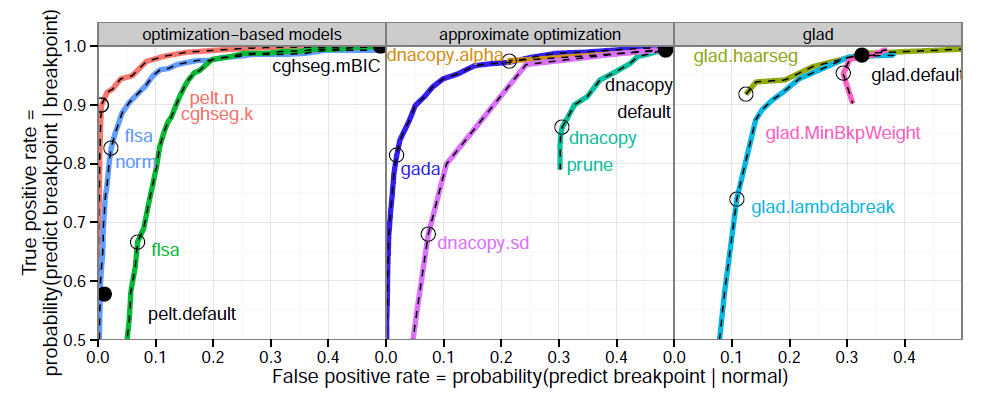
\epsfig{file = ../Figures/Hoc12-Fig3-3.eps, width=.95\textwidth}     \\
  \pause 
%   \vspace{-.5cm}
  \begin{itemize}
   \item DP and PELT clearly achieve the best performances.
   \item These two methods exactly the (penalized) likelihood maximization.
   \item But the choice of the number of segments remains an issue.
  \end{itemize}

 }

%====================================================================
\frame{\frametitle{Data transformation}

  \vspace{-3.5cm}
  \begin{tabular}{cc}
    \begin{tabular}{p{.4\textwidth}}
    \epsfig{file = ../Figures/p13.ps, clip=, width=.4\textwidth}     
    \end{tabular}
    &
    \begin{tabular}{p{.4\textwidth}}
    \epsfig{file = ../Figures/gene13.ps, clip=, width=.4\textwidth}     
    \end{tabular}
  \end{tabular}

  \vspace{-3.5cm}
  \begin{tabular}{cc}
    \begin{tabular}{p{.4\textwidth}}
    \epsfig{file = ../Figures/geneEFB1.ps, clip=, width=.4\textwidth}     
    \end{tabular}
    &
    \begin{tabular}{p{.4\textwidth}}
    \epsfig{file = ../Figures/EFG1.ps, clip=, width=.4\textwidth}     
    \end{tabular}
  \end{tabular} \\
  \Refer{Cleynen, 2012}
  }

%====================================================================
\frame{\frametitle{CGH-seg package}

  \paragraph{CGHseg} is an R package dedicated to the analysis of
  CGH profiles \refer{PLH11}.
  
  \bigskip\pause
  \paragraph{Linear model framework:} 
 
  \medskip
  \begin{tabular}{p{.2\textwidth}p{.35\textwidth}p{.35\textwidth}}
%     \emphase{Task} & \emphase{Representation} & \emphase{Model} \\   
%     \hline
%     \\
    \emphase{Segmentation} & regression on unknown $\Tbf$: &
    $\displaystyle{\Ybf = \Tbf \mubf + \Ebf}$ \pause \\ 
    \\
    \emphase{Correlation} & {factor model(\footnote{uniform
        correlation}): $\Zbf$}  & 
    $\displaystyle{\sl \Ybf = \Tbf \mubf + \Bbf \Zbf + \Ebf}$ \pause \\ 
    \\
    \emphase{Correction} & fixed covariates effect: $\betabf$ &
    $\displaystyle{\Ybf = \Tbf \mubf + \Xbf \betabf + \Ebf}$ \pause \\  
    \\
    \emphase{Calling} & cross-tabulation table $\Cbf$: &
    $\displaystyle{\Ybf = \Tbf \Cbf \mbf + \Ebf}$ \pause \\
    \\
    \emphase{Combinations} 
    & fixed + random effects: &
    $\displaystyle{\Ybf = \Tbf \mubf + \Xbf \betabf + \Lbf \Zbf + \Ebf}$ \\
    & fixed effects + calling: &
    $\displaystyle{\Ybf = \Tbf \Cbf \mbf + \Xbf \betabf + \Ebf}$  \\
  \end{tabular}
}

%====================================================================
\subsection*{Comparing change-points}
%====================================================================
\frame{\frametitle{A bit further: comparing change-points}

  \paragraph{Change-point location.} No method described until now gives information about the \emphase{precision of the change point location $\tau_k$} (confidence or credibility interval).

  \pause\bigskip\bigskip
  \paragraph{Credibility interval.} A quadratic ($O(Kn^2)$) algorithm can be designed to compute the (exact) posterior distribution of the change points.	
  $$
  \epsfig{file=../Figures/Bayes-data.ps, clip=, width=1\textwidth, bburx=515, bbury=315, bbllx=0, bblly=210}
  $$

  }

%====================================================================
\frame{\frametitle{Change-point comparison}

  \begin{tabular}{cc}
    \hspace{-.5cm}
    \begin{tabular}{p{.5\textwidth}}
      \onslide+<1->{
        \paragraph{Change-point location}
        \begin{itemize}
        \item Comparison \textcolor{red}{posterior} vs \\
          \textcolor{blue}{'official' annotation}
        \end{itemize} 
	~\\
        }
      \onslide+<2->{
        \paragraph{Comparison}
        \begin{itemize}
        \item Posterior distribution under different conditions can be compared.
        \item Providing a statistical assessment of transcription starting sites variations.
        \end{itemize}
        }
    \end{tabular}
    & 
    \hspace{-1.3cm} 
    \begin{tabular}{p{.5\textwidth}}
      %\vspace{-.5cm}
      \begin{overprint}
        \onslide<1>
	\epsfig{file=../Figures/Bayes-data.ps, clip=, width=.5\textwidth, height=.9\textheight}
%         \includegraphics[width=.5\textwidth, height=.9\textheight]{../Figures/Bayes-data} 
        \onslide<2->
	\epsfig{file=../Figures/compa-end.ps, clip=, width=.5\textwidth, height=.4\textheight, bbllx=40, bblly=50, bburx=500, bbury=210}
%         \includegraphics[width=.5\textwidth, height=.9\textheight]{../Figures/compa-end}
      \end{overprint}
    \end{tabular}
  \end{tabular}
}

%====================================================================
\section{Hidden Markov model}
\frame{\frametitle{Hidden Markov model}}
\label{Page:HMM}
%====================================================================

%====================================================================
\frame{\frametitle{Back to the the basic problem}
  
  %\vspace{-0.5cm}
  \begin{tabular}{cc}
    \begin{tabular}{p{.5\textwidth}}
      \onslide+<1->{We wanted to go from there \\}
      \onslide+<2->{... to there. \\ ~\\
  Methods presented until no provide estimates of the change-point location and of the mean signal in each segment. \\ ~\\}
      \onslide+<3->{But we still miss the text, that is, the 'calling'.}
    \end{tabular}
    &
    \begin{tabular}{p{.5\textwidth}}
      \hspace{-1cm}
      \begin{overprint}
        \onslide<1>
        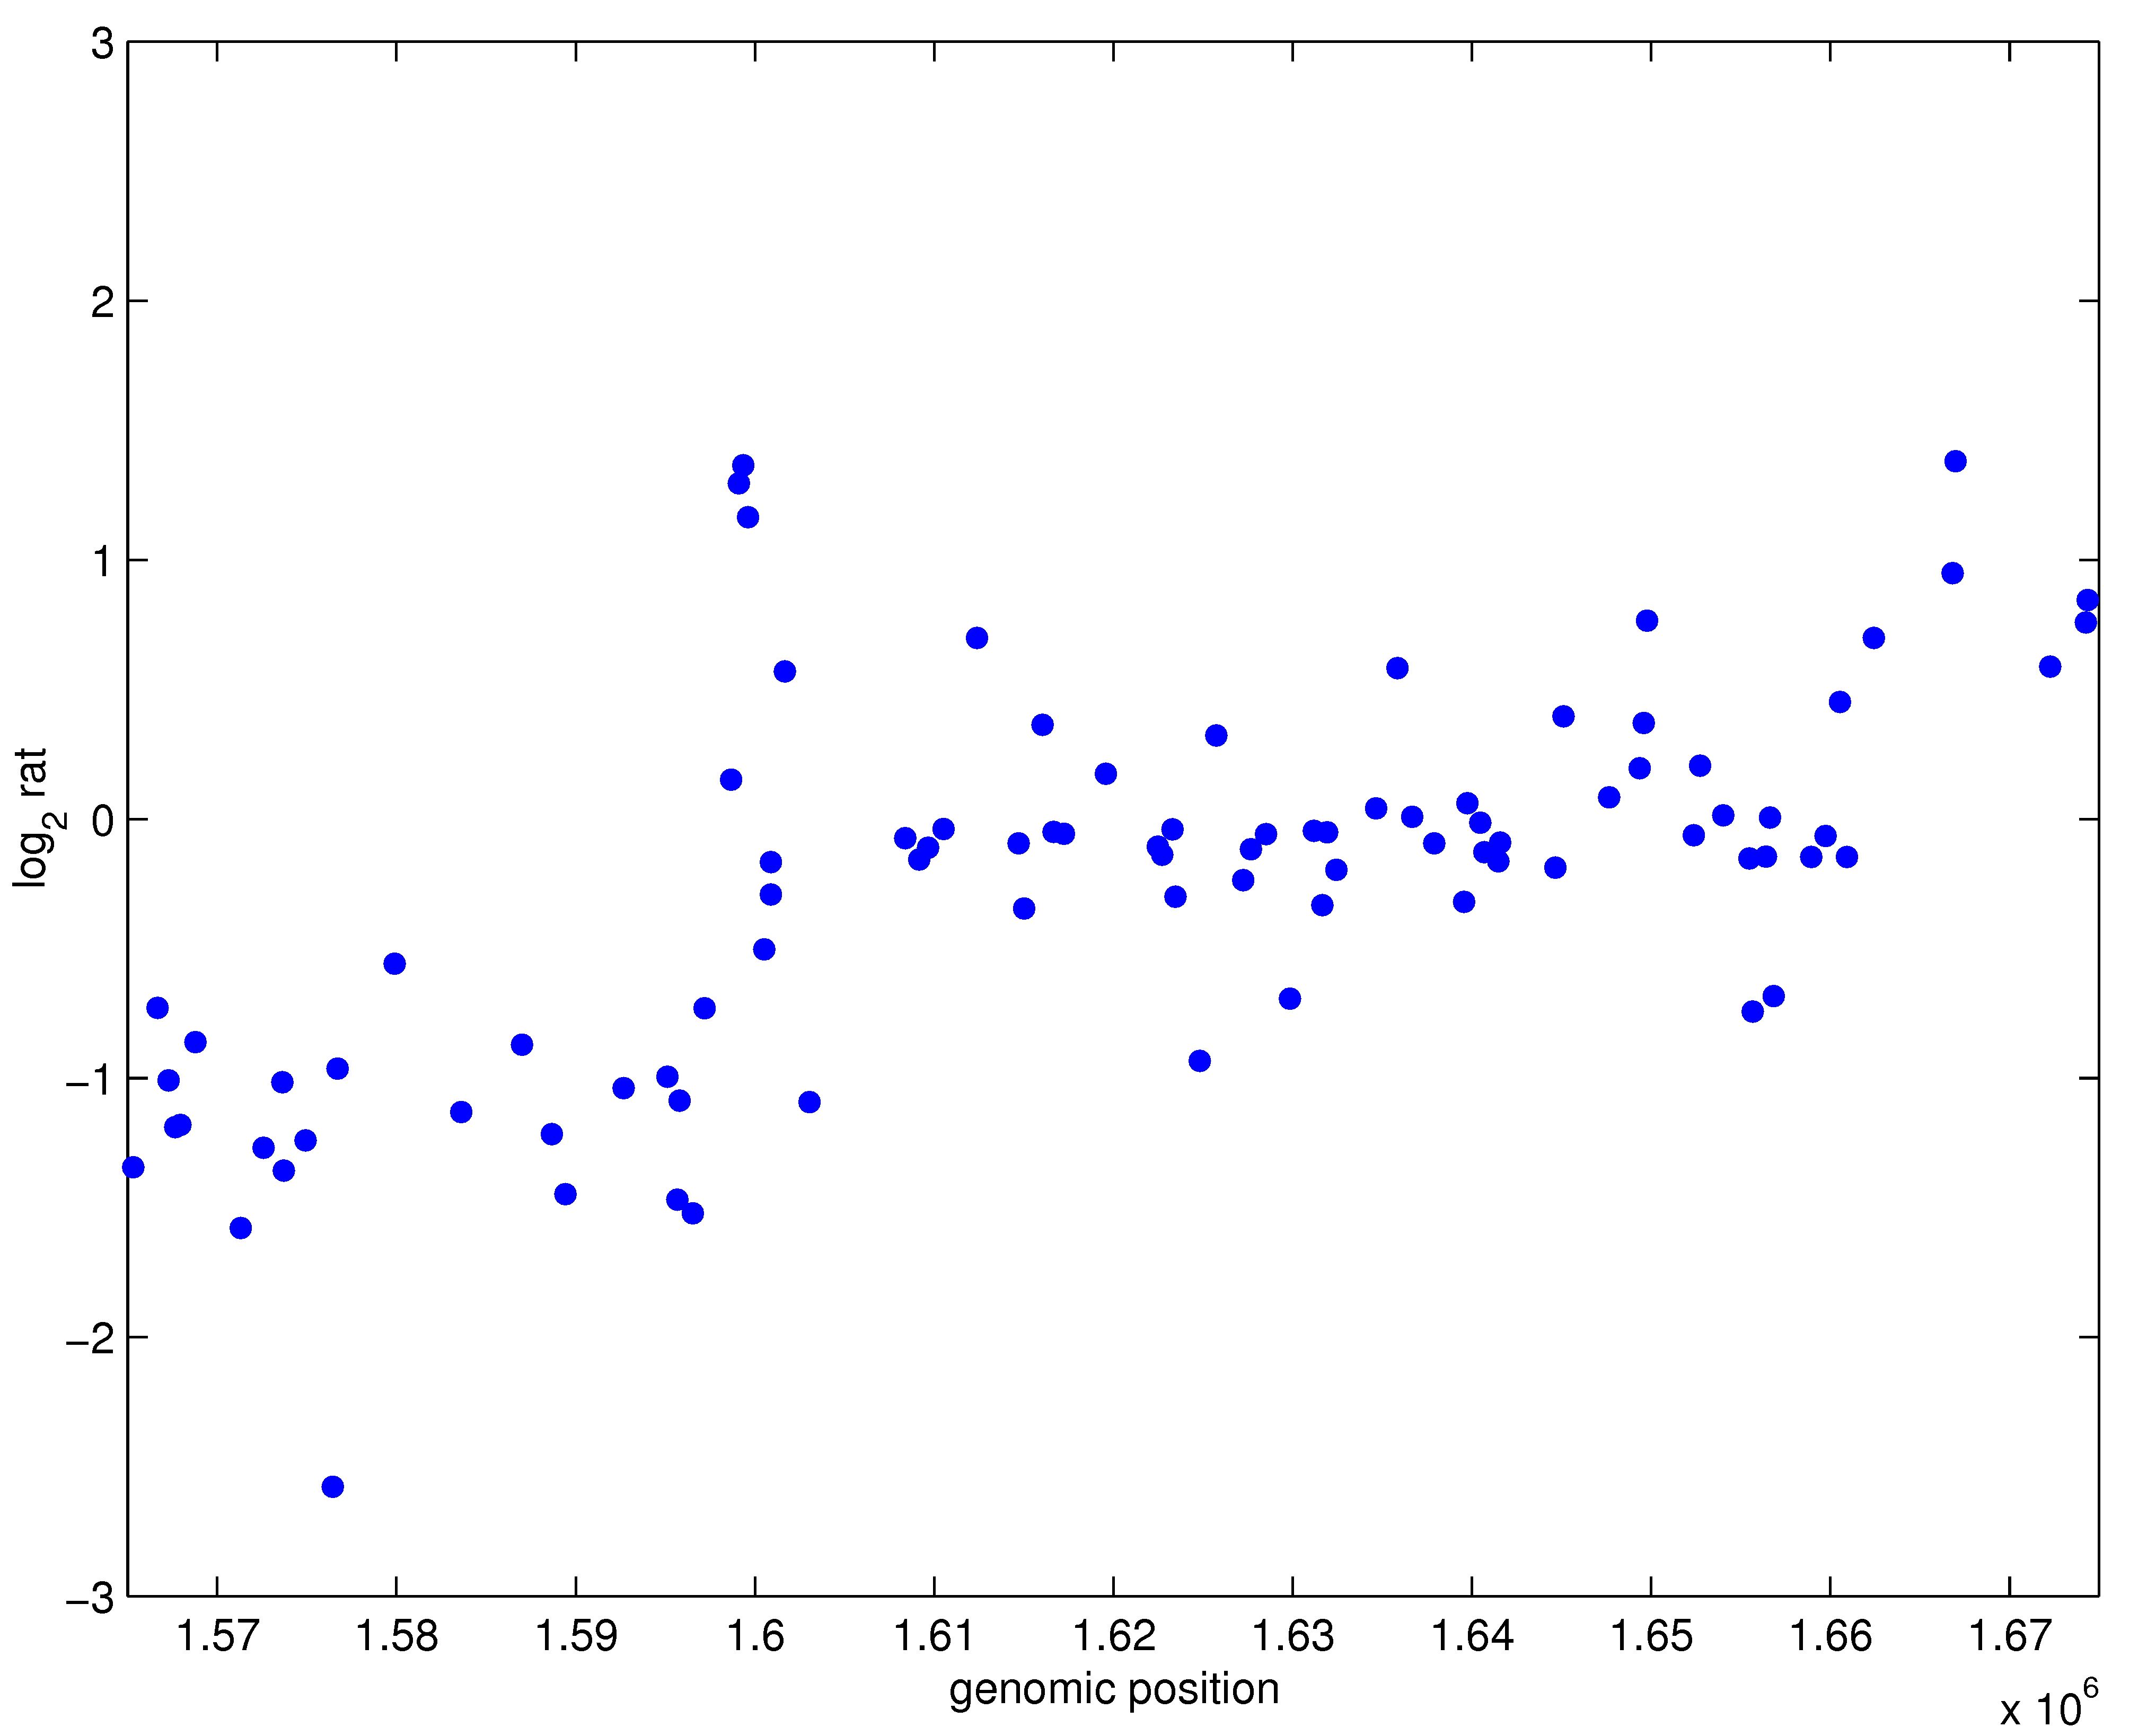
\epsfig{file = ../Figures/raw_profile_example.eps, clip=,
          width=.45\textwidth, height=.5\textheight}  
        \onslide<2->
        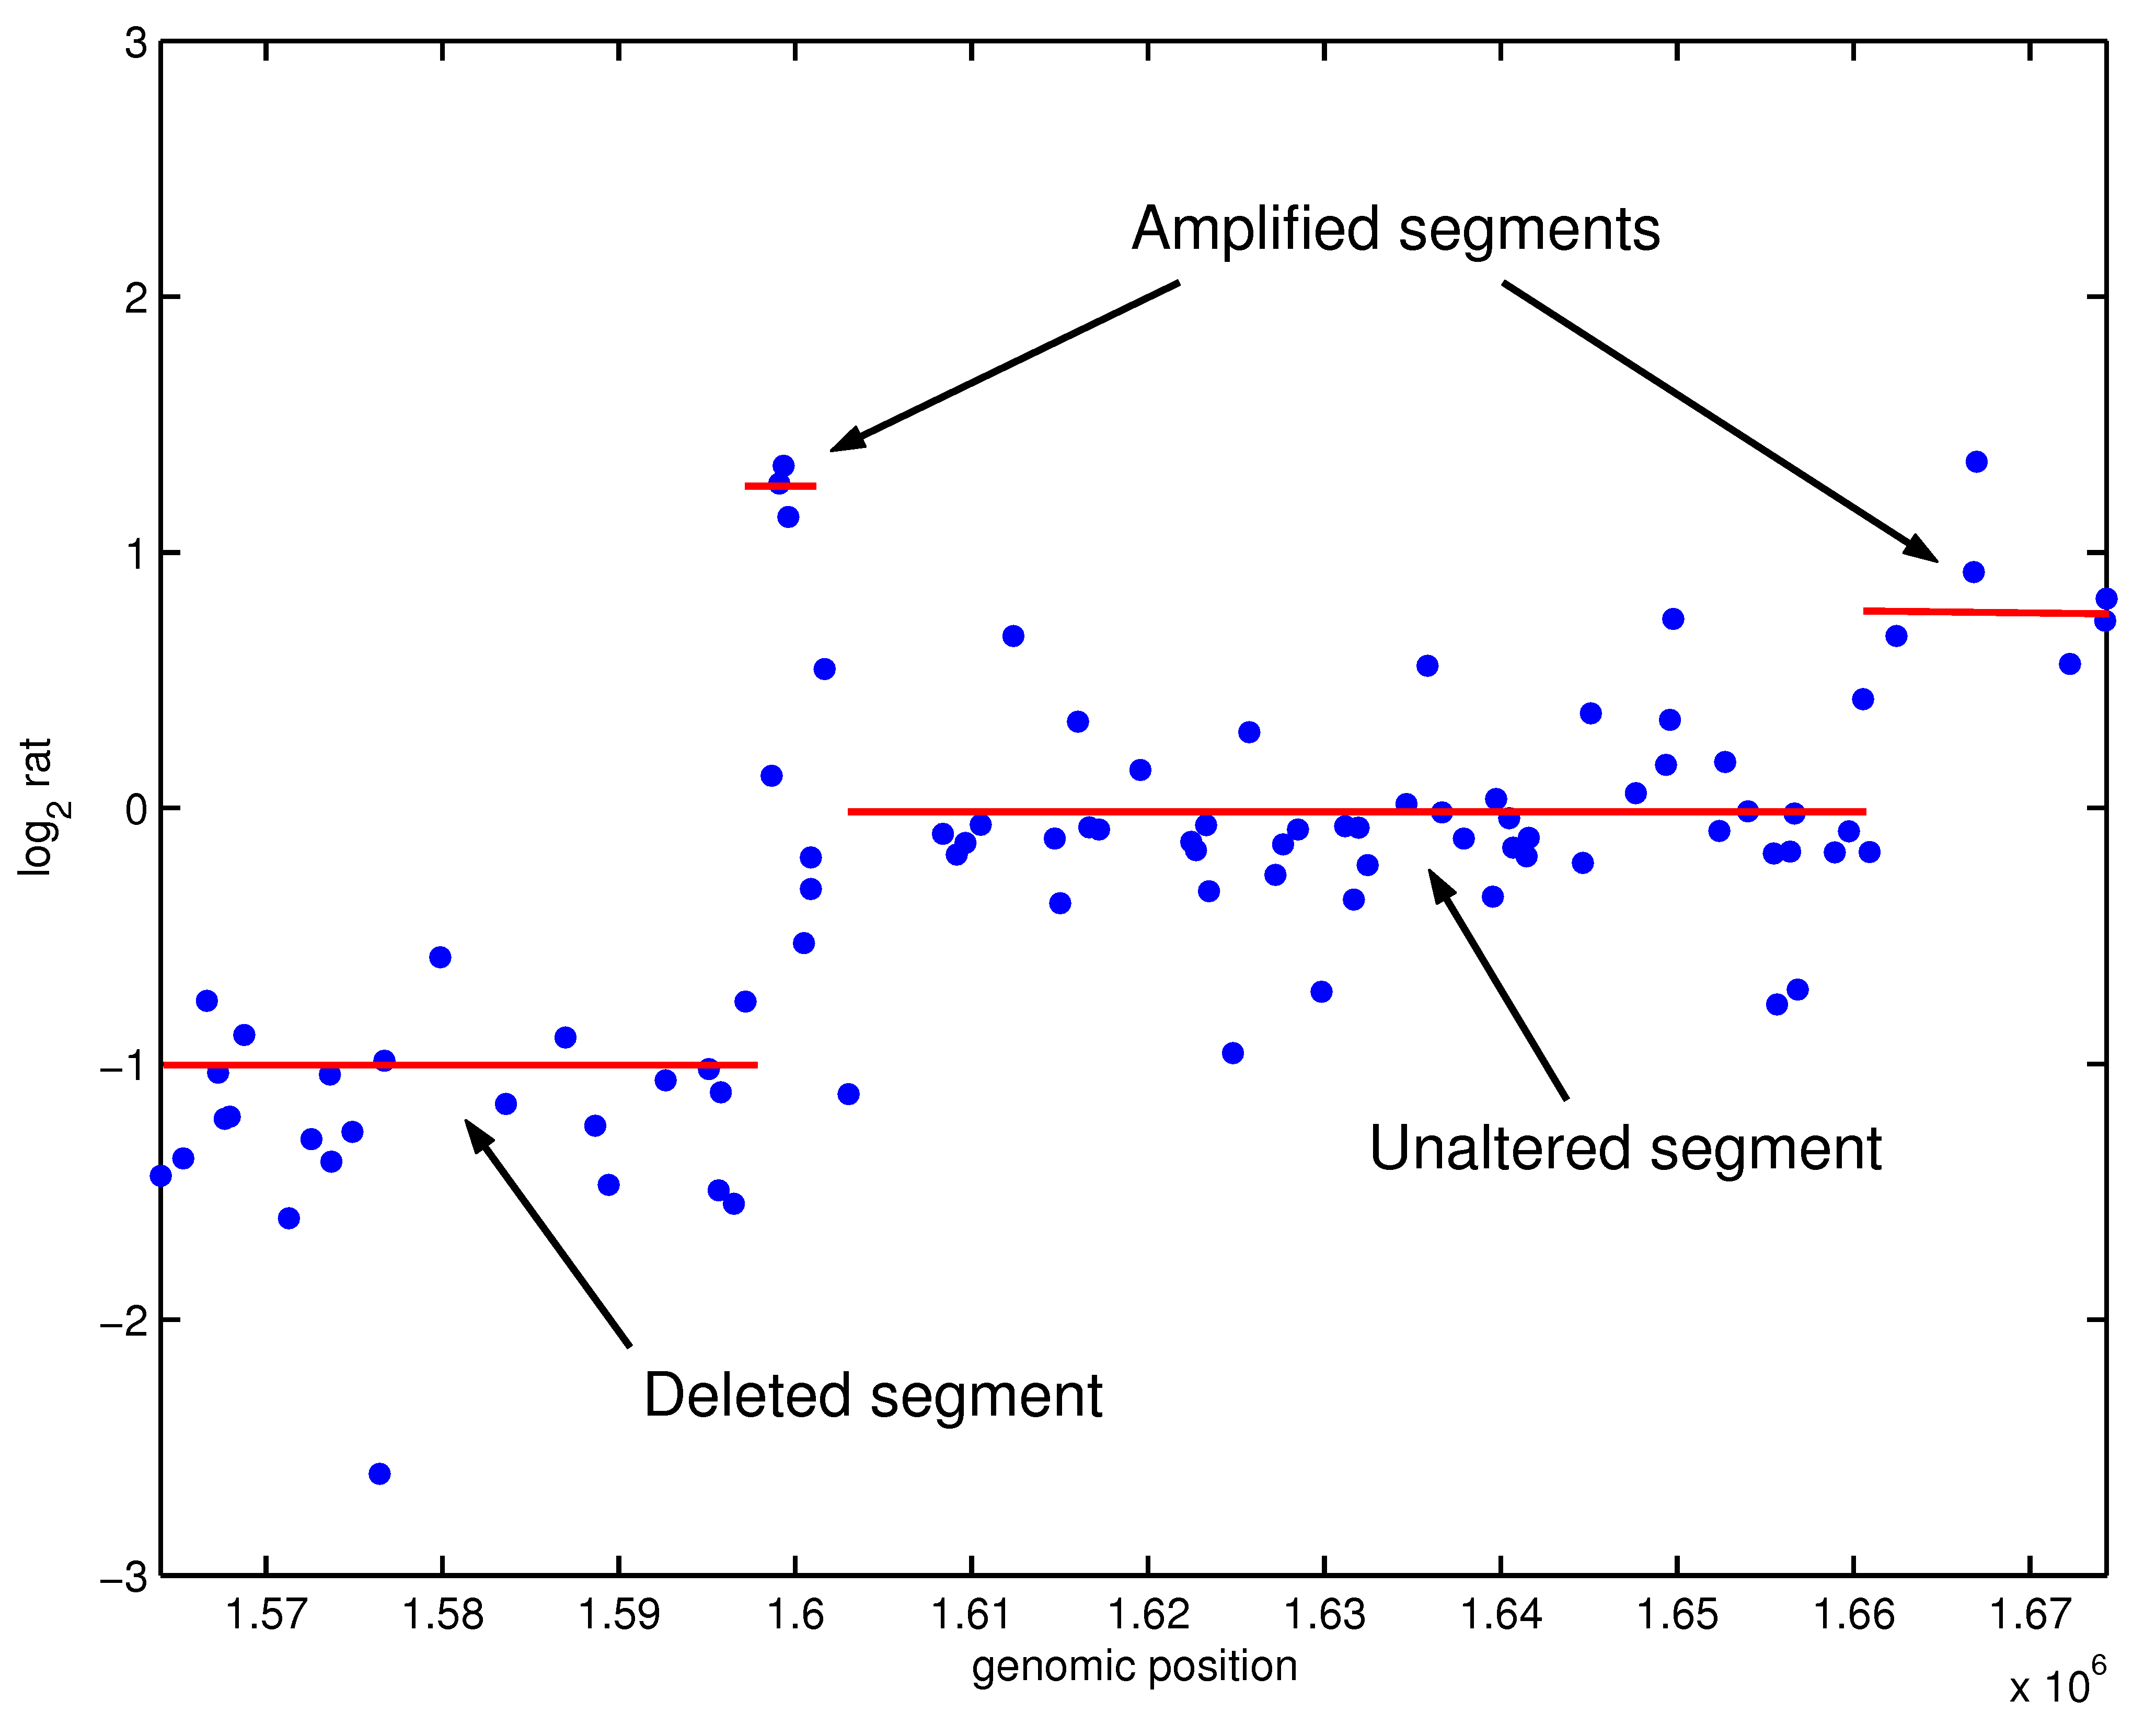
\epsfig{file = ../Figures/profile_example.eps, clip=,
          %bbllx=60, bblly=196, bburx=543, bbury=586}
          width=.45\textwidth, height=.5\textheight}  
      \end{overprint}
    \end{tabular}
  \end{tabular} \\
   
  }

%====================================================================
\frame{\frametitle{Another model for the same problem}

  \vspace{-0.5cm}
  \begin{tabular}{cc}
    \hspace{-1cm}
    \begin{tabular}{p{.5\textwidth}}
      \begin{itemize}
      \item \onslide+<1->{$t = 1..n$ probes (positions) are observed.}
      \item \onslide+<2->{An \emphase{unobserved label $Z_t$}
          ('loss', '\textcolor{red}{normal}',
          '\textcolor{darkgreen}{gain}') is associated with each probe;}
      \item \onslide+<3->{The distribution of the \emphase{observed signal
          $Y_t$} depends on the label.}
      \item \onslide+<4->{We only observe the signal;}
      \item \onslide+<5->{And we would like to retrieve the 'truth'.}
      \end{itemize}
    \end{tabular}
    &    \hspace{-1cm}
    \begin{tabular}{p{.5\textwidth}}
      \begin{overprint}
        \onslide<1> 
        \epsfig{file=\figSimHMM/SimHMM_n100_Q3.eps,
          width=0.4\textwidth, height=0.7\textheight, angle=270, clip=}
        \onslide<2> 
        \epsfig{file=\figSimHMM/SimHMM_n100_Q3_Z.eps,
          width=0.4\textwidth, height=0.7\textheight, angle=270, clip=}
        \onslide<3> 
        \epsfig{file=\figSimHMM/SimHMM_n100_Q3_ZX.eps,
          width=0.4\textwidth, height=0.7\textheight, angle=270, clip=}
        \onslide<4> 
        \epsfig{file=\figSimHMM/SimHMM_n100_Q3_X.eps,
          width=0.4\textwidth, height=0.7\textheight, angle=270, clip=}
        \onslide<5> 
        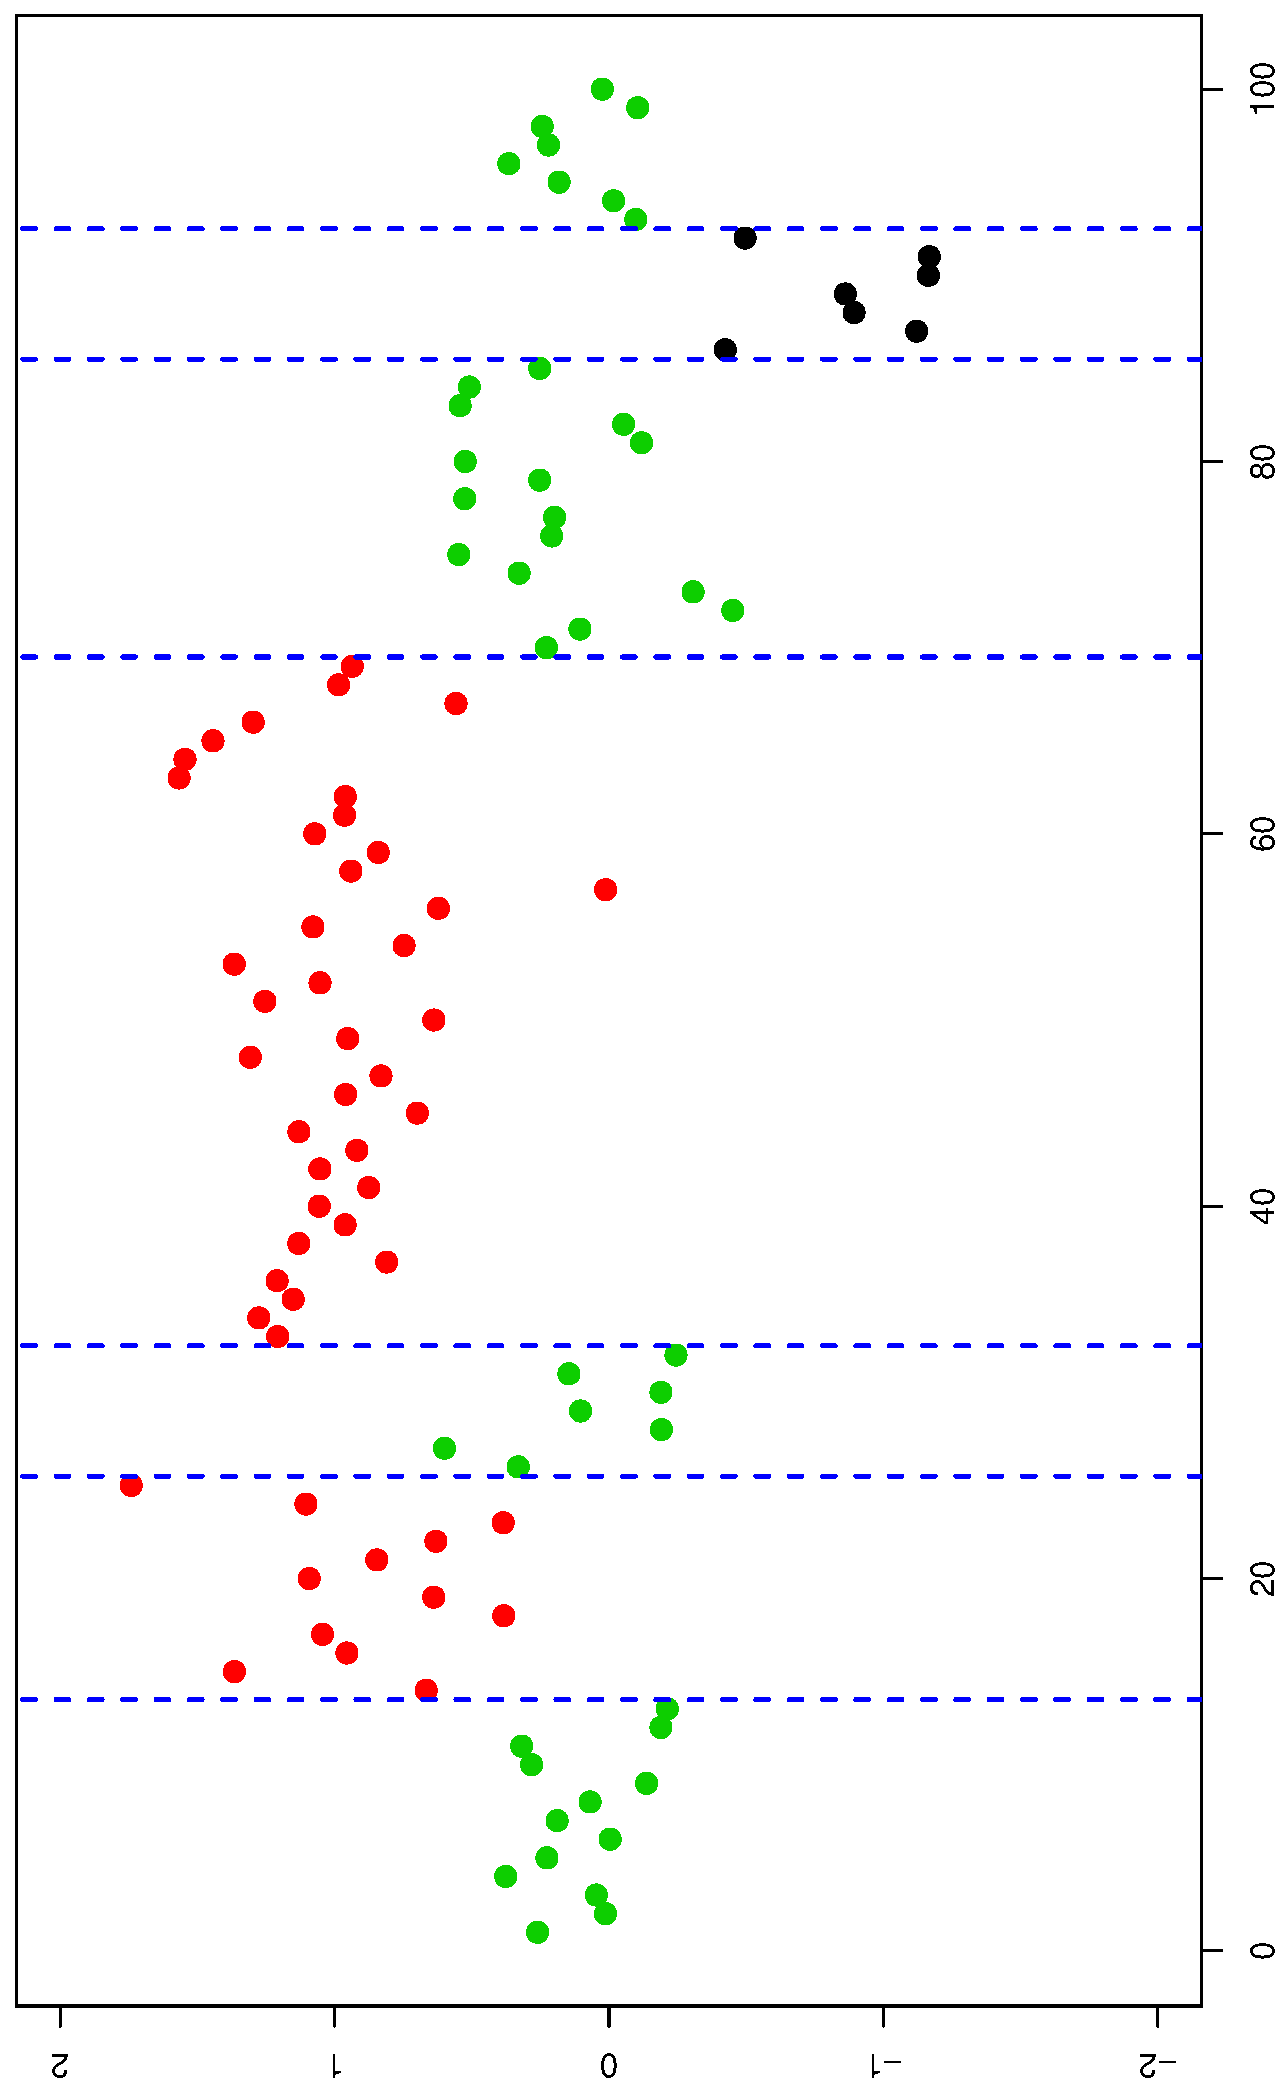
\epsfig{file=\figSimHMM/SimHMM_n100_Q3_ZvitXT.eps,
          width=0.4\textwidth, height=0.7\textheight, angle=270, clip=}
        \onslide<6> 
        \epsfig{file=\figSimHMM/SimHMM_n100_Q3_ZXT.eps,
          width=0.4\textwidth, height=0.7\textheight, angle=270, clip=}
      \end{overprint}
    \end{tabular}
  \end{tabular} \\
  \onslide+<6->{(Although we know we won't succeed.)}
  
}

%====================================================================
\frame{\frametitle{Statistical model}

  \onslide+<1->{
    \paragraph{Hidden labels.} $(Z_t)$ is a Markov chain:
    \begin{itemize}
    \item $Z_t \in \emphase{\{1..Q\}}$, e.g. $Q = 3$ for
      $\{$'loss', 'normal', 'gain'$\}$;
    \item The label of a probe \emphase{depends on the label of the
        preceding} probe:
      $$
      \text{transition probability} \quad \pi_{q\ell} = 
      \Pr\{Z_t = \ell | Z_{t-1} = q\}
      $$
    \end{itemize}
    }
    
    \onslide+<2->{
      \bigskip
      \paragraph{Observed signal.} $(Y_t)$ are independent, given the
      labels $(Z_t)$:
      $$
      \text{if } Z_t = q: \qquad
      Y_t \sim \Ncal(\mu_q, \sigma^2_{(q)})
      \qquad \text{or} \qquad
      Y_t \sim \Pcal(\mu_q).
      $$
    }
    
    \paragraph{Graphical model representation.}
    \begin{overprint}
      \onslide<1>
      $$
      \epsfig{file=../Figures/GM-HMM-ZY.eps,
        bbllx=0, bblly=465, bburx=660, bbury=540,
        width=0.7\textwidth, clip=}
      $$
      \onslide<2>
      $$
      \epsfig{file=../Figures/GM-HMM-ZY.eps,
        bbllx=0, bblly=335, bburx=660, bbury=540,
        width=0.7\textwidth, clip=}
      $$
    \end{overprint}
  }

%====================================================================
\frame{\frametitle{Parameter inference}

  \paragraph{Incomplete data model.} Parameter inference would be easy
  if the labels where known.

  \bigskip\pause
  \paragraph{E-M algorithm.} The most common strategy consist in
  retrieving the missing information.
  \begin{itemize}
  \item \emphase{E-step:} Compute (in linear time) the probability for each probe $t$
    to have label $q$ (forward-backward algorithm):
    $$
    \tau_{tq} = \Pr\{Z_t = q \;|\; \Ybf\};
    $$
  \item \pause \emphase{M-step:} Estimate the parameters based the
    inferred labels, e.g.
    $$
    \widehat{\mu}_q = \sum_t \tau_{tq} Y_t \left/ \sum_t \tau_{tq} \right..
    $$
  \end{itemize}
  \refer{DLR77}, \refer{CMR05}, \refer{DEK99}
  }

%====================================================================
\frame{\frametitle{Classification = 'Calling'}

  \onslide+<1->{
    \paragraph{Probe classification.} Segmentation is finally obtained
    by assigning a label to each probe.
  }
  
  \bigskip
  \begin{tabular}{cc}
    \hspace{-0.5cm}
    \begin{tabular}{p{.5\textwidth}}
      \onslide+<2->{
        \paragraph{MAP rule.} 
        The $\tau_{tq}$ can provide \emphase{maximum a posteriori}
        classification:
        $$
        \widehat{Z}_t = \arg\max_q \tau_{tq}.
        $$ \\
      }
      \onslide+<3->{
        \paragraph{Most probable hidden path.} The succession of the
        MAP $(\widehat{Z}_t)$ is \emphase{not} the most probable
        hidden path ('Viterbi path'):
        $$
        \widehat{\Zbf} = \arg\max_{\Zbf} p(\Zbf|\Ybf) \neq
        (\widehat{Z}_t) 
        $$
        % \begin{eqnarray*}
        %   \widehat{\Zbf} & = & \arg\max_{\Zbf} p(\Zbf|\Ybf) \\
        %   & \neq & (\widehat{Z}_t) 
        % \end{eqnarray*}
      }
    \end{tabular}
    &
    \hspace{-1cm}
    \begin{tabular}{p{.5\textwidth}}
      \begin{overprint}
        \onslide<1> 
        \epsfig{file=\figSimHMM/SimHMM_n100_Q3_X.eps,
          width=0.4\textwidth, height=0.7\textheight, angle=270, clip=}
        \onslide<2> 
        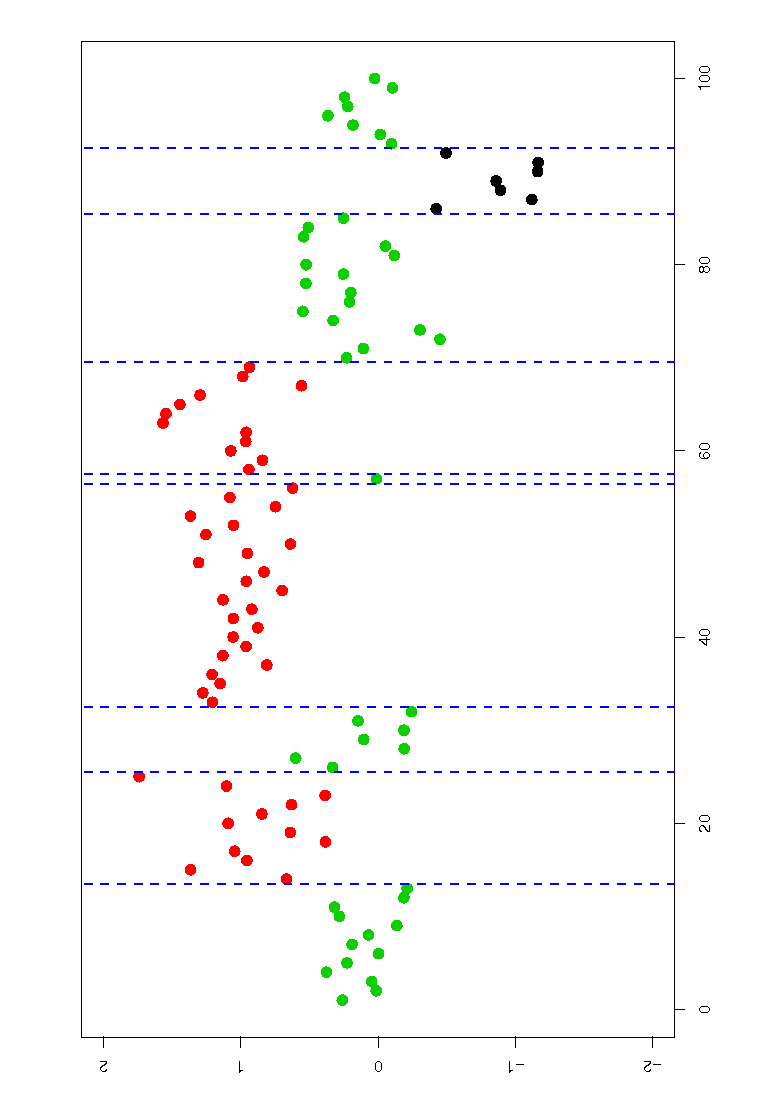
\epsfig{file=\figSimHMM/SimHMM_n100_Q3_ZmapXT.eps,
          width=0.4\textwidth, height=0.7\textheight, angle=270, clip=}
        \onslide<3> 
        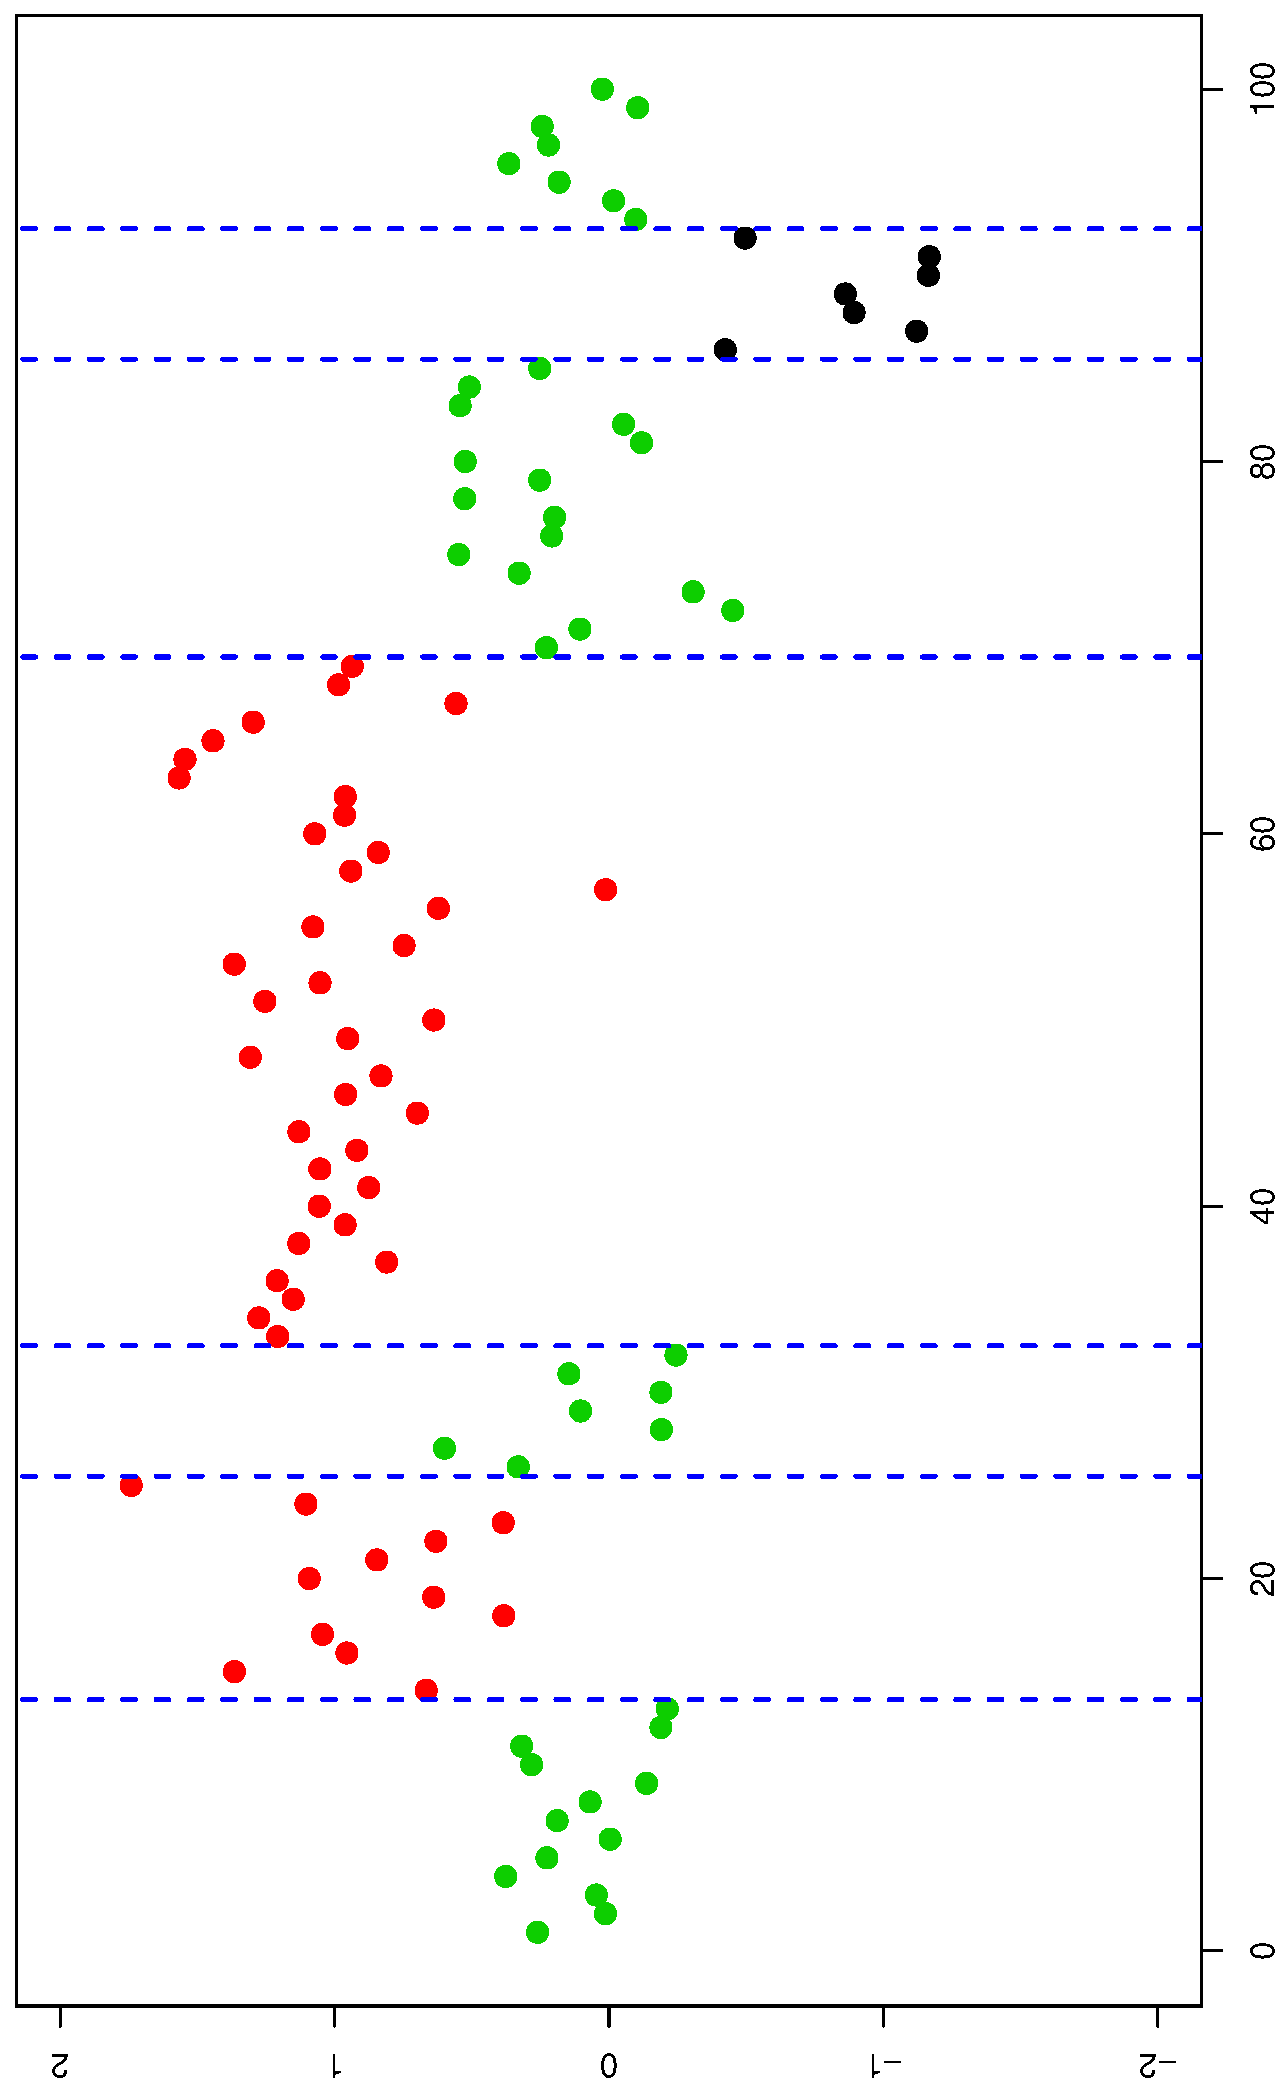
\epsfig{file=\figSimHMM/SimHMM_n100_Q3_ZvitXT.eps,
          width=0.4\textwidth, height=0.7\textheight, angle=270, clip=}
      \end{overprint}
    \end{tabular}
  \end{tabular}
  
  }

%====================================================================
\frame{\frametitle{Issues}

  \paragraph{Algorithmics.} 
  \begin{itemize}
  \item The conditional distribution of the labels given the
    observation $\emphase{p(\Zbf | \Ybf)}$ is not explicit;
  \item But it can be computed \emphase{in a linear time $O(nK^2)$}
    with the forward-backward algorithm.
  % \item The most probable hidden path $\widehat{\Zbf} = \arg\max
  %   p(\Zbf | \Ybf)$ can be computed with the same complexity with
  %   the Viterbi algorithm.
  \end{itemize}
  
  \bigskip\pause
  \paragraph{Statistics.}
  \begin{itemize}
  \item The E-M algorithm aims at computing the maximum-likelihood
    estimates;
  \item But its behavior strongly depends on the starting point...
  \item The Markov assumption has some consequences on the
    distribution of the length of the segments.
  \end{itemize}
  
  \bigskip\pause
  \paragraph{Model selection.}
  \begin{itemize}
  \item The number of hidden classes $Q$ is unknown;
  \item But is often chosen with standard criteria, such as BIC.
  \end{itemize}
}

%====================================================================
%====================================================================
\section{LASSO approaches}
\frame{\frametitle{LASSO approaches}}
%====================================================================


%====================================================================
\subsection*{Convex optimization}
%====================================================================
\frame{\frametitle{An optimization perspective} 

  \vspace{-0.5cm}
  \begin{tabular}{cc}
    \hspace{-0.5cm}
    \begin{tabular}{p{.6\textwidth}}
      \paragraph{Segmentation problem} can be rephrased as
      $$
      \widehat{\mubf}_{\text{Seg}} = \min_{\mubf} \sum_t (Y_t - \mu_t)^2 
      + \lambda \sum_t |\mu_t - \mu_{t-1}|_0 
      $$
      where $|\cdot|_0$ stands for the so-called $\ell_0$ norm:
    \end{tabular}
    &
    \hspace{-1cm}
    \begin{tabular}{p{.35\textwidth}}
      \epsfig{file=../Figures/FigSeg-Budapest-4.eps, clip=,
        angle=270, width=.4\textwidth}       
    \end{tabular}
  \end{tabular}
  \vspace{-.5cm}
  $$
  \sum_t |\mu_t - \mu_{t-1}|_0 = \text{\emphase{number of changes} in
    $\mu_t$} = K-1
  $$
  and $\lambda$ controls the number of segments $K$.
  
  \pause\bigskip
  \paragraph{Remarks.}
  \begin{itemize}
  \item This optimization problem turns out to be
    \emphase{non convex}. 
  \item This prevents the use the huge set of \emphase{convex
      optimization} techniques.
  \item Hopefully, dynamic programming does exist.
  \end{itemize}
}\label{Page:Lasso}

%====================================================================
\frame{\frametitle{Lasso}

  \paragraph{Lasso trick.} Replacing the $\ell_0$ with the
  $\ell_1$ norm makes the optimization problem convex:
  $$
  \widehat{\mubf}_{\text{Lasso}} = \min_{\mubf} \sum_t (Y_t - \mu_t)^2 
  + \lambda \sum_t |\mu_t|
  $$
  that can be solved in \emphase{linear time}.

  \bigskip
  %\vspace{-0.5cm}
  \begin{tabular}{cc}
    \hspace{-0.5cm}
    \begin{tabular}{p{.5\textwidth}}
      \onslide+<2->{
        \paragraph{Regularization:} \\
      }
      \begin{itemize}
        \onslide+<3->{
        \item Due to the $\ell_1$ topology, most of the parameters
          $\mu_t$ are \emphase{set to 0}. \\ ~
        } 
        \onslide+<4->{
        \item The coefficient $\lambda$ controls the \emphase{number of
          non-zero terms}. \\ ~
          }
      \end{itemize}
      \vspace{2cm}
      ~
    \end{tabular}
    &
    \hspace{-.5cm}
    \begin{tabular}{p{.5\textwidth}}
      \begin{overprint}
        \onslide<2>
        \epsfig{file=../Figures/Reg-Lasso0-mu.eps, clip=,
          width=0.6\textwidth}
        \onslide<3>
        \epsfig{file=../Figures/Reg-Lasso1-mu.eps, clip=,
          width=0.6\textwidth}
        \onslide<4->
        \epsfig{file=../Figures/Reg-Lasso2-mu.eps, clip=,
          width=0.6\textwidth}
      \end{overprint}
    \end{tabular}
  \end{tabular}
}

%====================================================================
\frame{\frametitle{Fused Lasso}

  \paragraph{Fused Lasso.} For a segmentation purpose, a second term
  penalizing \emphase{changes among the $\mu_t$} can be added
  (\refer{TSR05}):
  $$
  \widehat{\mubf} = \min_{\mubf} \sum_t (Y_t - \mu_t)^2 
  + \lambda_1 \sum_t |\mu_t| 
  + \lambda_2 \sum_t |\mu_t - \mu_{t-1}| 
  $$
  $$
  \text{where } \sum_t |\mu_t - \mu_{t-1}|_1 = \text{\emphase{sum of
      the absolute changes} in $\mu_t$.}
  $$
  
  \bigskip\pause
  \paragraph{Interpretation.}
  \begin{itemize}
  \item $\sum_t (Y_t - \mu_t)^2$: fit to the observations;
  \item $\lambda_1 \sum_t |\mu_t|$: controls the number of 'abnormal' positions;
  \item $\lambda_2 \sum_t |\mu_t - \mu_{t-1}|$: controls the number of
    breakpoints.
  \end{itemize}
}
 
%====================================================================
\frame{\frametitle{Application to CGH}

  \paragraph{Effect of $w = 2 \lambda_1 / \lambda_2$.}  \refer{TiW08}
  \\ ~\\
  
  \begin{tabular}{c}
    \epsfig{file=../Figures/TiW07-BioStat-Fig2.ps, clip=,
      bblllx=0, bblly=630, bburx=690, bbury=756, 
      width=0.9\textwidth} \\ \pause
    \epsfig{file=../Figures/TiW07-BioStat-Fig2.ps, clip=,
      bblllx=0, bblly=440, bburx=690, bbury=560, 
      width=0.9\textwidth} \\ \pause
    % \epsfig{file=../Figures/TiW07-BioStat-Fig2.ps, clip=,
    %   bblllx=0, bblly=250, bburx=690, bbury=370, 
    %   width=0.9\textwidth} \\ \pause
    \epsfig{file=../Figures/TiW07-BioStat-Fig2.ps, clip=,
      bblllx=0, bblly=55, bburx=690, bbury=180, 
      width=0.9\textwidth} \\
  \end{tabular}
  }

%====================================================================
%====================================================================
\section*{Conclusion}
%====================================================================
\frame{\frametitle{To end}

  \paragraph{R packages.}
   \begin{description}
   \item[CGHseg:] Comprehensive package for joint segmentation of multiple profile (+ between profiles correlation + bias correction + calling)
   \item[EBS:] Exact posterior distribution for segmentation (model selection, credibility intervals, ...) for both microarray and NGS
   \item[Segmentator3IsBack:] Pruned dynamic programming for efficient segmentation of large signals (microarray, NGS)
   \end{description}

  \bigskip \bigskip \pause
  \paragraph{Acknowledgements.}
  A. Cleynen, S. Huet, E. Lebarbier, F. Picard, G. Rigaill
}
%====================================================================
%====================================================================
\subsection*{References}
%====================================================================
{\tiny
  \bibliography{/media/donnees/Biblio/ARC,/media/donnees/Biblio/AST,/media/donnees/Biblio/SSB}
  \bibliographystyle{/media/donnees/LATEX/astats}
  %\bibliographystyle{plain}
  }

%====================================================================
%====================================================================
\end{document}
%====================================================================
%====================================================================


\frame{\frametitle{}
  }

  \vspace{-0.5cm}
  \begin{tabular}{cc}
    \hspace{-0.5cm}
    \begin{tabular}{p{.5\textwidth}}
    \end{tabular}
    &
    \hspace{-1cm}
    \begin{tabular}{p{.5\textwidth}}
    \end{tabular}
  \end{tabular}
